%Copyright FG Mauthe, University of Koblenz-Landau, Koblenz, Germany
% v1.0, last changed 19.04.21

\documentclass[%
	BCOR=8mm, % Bindekorrektur
	DIV=12,
	toc=bibliography, % references in contents
	toc=listof, % list of tables and figures in contents
	oneside, %use twoside if preferred
	egregdoesnotlikesansseriftitles, % deletes the usage of sffamily font
	]{scrbook}

% Set the font right away, this is global, egregdoesnotlikesansseriftitles is already set, but overwritten with this command
\renewcommand{\familydefault}{\sfdefault} % bfseries

% Alternative, needs to be adjusted
%\documentclass[a4paper, twoside]{article}

%\newlength{\laenge}
%\setlength{\laenge}{2mm}
%\setlength{\parindent}{2\laenge}

\usepackage{xcolor}
\pagecolor{white} % white pages

% Font / Formatting packages
\usepackage[latin1]{inputenc}   % font-coding
\usepackage{listingsutf8}
\usepackage{caption}
\usepackage{subfigure}
\usepackage{parskip}
%\usepackage{cite}
\usepackage{lmodern}
\usepackage{multirow}
% Use either English or German
\usepackage[english]{babel}
%\usepackage[ngerman]{babel}

% Math packages
\usepackage{amsmath} % math package
\usepackage{amsfonts} % for additional mathematical symbols
\usepackage{dsfont} % double stroke fonts, for instance to depict the natural numbers symbol |N

% More useful packages
\usepackage{float} % for "containers"
\usepackage{url}
\usepackage[onehalfspacing]{setspace} % simple option to change the spacing
\usepackage{layout}
\usepackage{fancyhdr}	% header
\usepackage{graphicx}
\usepackage{booktabs} % For prettier tables
\usepackage{chngcntr} % enables the additional numbering of figures and tables
\usepackage{hyperref} % for clickable and marked cross references
%\usepackage{pdfpages}
\usepackage{forest}
\usepackage{algorithm}
\usepackage{algorithmic}

\usepackage[
backend=biber,
style=numeric-comp,
]{biblatex}

\addbibresource{references.bib}


% APPENDIX
\usepackage[toc,page]{appendix} % in case you'd like to use an appendix

\begin{document}

% Title Page
% Copyright FG Mauthe, University of Koblenz-Landau, Koblenz, Germany
% Apply the necessary changes to make this page your own

\begin{titlepage}
	
\includegraphics[height=35pt]{img/uni-logo.png}
	\hfill
	
\includegraphics[height=35pt]{img/iwvi.jpg}

	\begin{center}
	\vspace{2.5cm}	
	
	\huge\textbf{Assessment of Mean Teacher and Prominent Adversarial Unlabeled Data for Language Classification}
	
	%\vspace{2cm}


	\normalsize
	\vspace{1.5cm}	

	\textsc{\Large Masterarbeit}\\Master of Science (M.Sc.) im Web and Data Science\\[2cm] 
		
	vorgelegt von\\
	
	\textbf{\Large Bhupender Kumar Saini}\\ $ [ $219 100 887$ ] $\\ [1.5cm] 
	
	Koblenz, im February 2022
	\end{center}
	\vfill
	\begin{tabular}{ll}
		Erstgutachter: & Prof. Dr. Andreas Mauthe\\ 
		 & \small{(Institut f\"ur Wirtschafts- und Verwaltungsinformatik, FG Mauthe)}\\
		Zweitgutachter: & Alexander Rosenbaum, M. Sc. \\ 
		& \small{(Institut f\"ur Wirtschafts- und Verwaltungsinformatik, FG Mauthe)}\\
		%Ggf. ext. Betreuer eintragen.
		%Betreuer:  & Max Mustermann, M.Sc.
	\end{tabular}
\end{titlepage}


% Student's declaration
% Copyright FG Mauthe, University of Koblenz-Landau, Koblenz, Germany

% Declaration
% ===> Do NOT CHANGE anything here

\pagestyle{empty}
\begin{quote}
	\textbf{\Large Eidesstattliche Erkl\"arung}

	Ich versichere, dass ich die vorliegende Arbeit selbst\"andig verfasst
	und keine anderen als die angegebenen Quellen und Hilfsmittel benutzt habe
	und dass die Arbeit 
	in gleicher oder \"ahnlicher Form noch keiner anderen Pr\"ufungsbeh\"orde
	vorgelegen hat und von dieser als Teil einer Pr\"ufungsleistung
	angenommen wurde. 
	\\[10mm]

	\begin{tabular}{@{}p{0.82\linewidth}@{\hspace*{2ex}}r@{\hspace*{2ex}}r}
		Mit der Einstellung der Arbeit in die Bibliothek bin ich einverstanden.
		& ja $\square$ & nein $\square$ \\[1em] 
		Der Ver\"offentlichung dieser Arbeit im Internet stimme ich zu.
		& ja $\square$ & nein $\square$ \\
	\end{tabular}
	\\[20mm]


	\dotfill
	\\(Ort, Datum) \hspace{8.5cm} (Unterschrift)
\end{quote}


% Abstract in German and English language
% According to the HPA (examination office) you are obligated to write
% an abstract in English and German

\pagestyle{plain}
\pagenumbering{Roman}

% Abstract DE
\begin{quote}
\textbf{\Large Zusammenfassung}\\\\
Sprachmodelle haben bei verschiedenen Aufgaben der natürlichen Sprachverarbeitung Spitzenleistungen gezeigt. Die Forschung hat gezeigt, dass ihre Modelle anfällig für feindliche Angriffe sind, bei denen unmerkliches Rauschen im Text ihre Leistung unerwartet beeinträchtigen kann. Darüber hinaus ist die Erforschung von Verteidigungsmechanismen ein vergleichsweise weniger erforschtes Thema als die Generierung prominenter Angriffe. In dieser Masterarbeit wird ein halbüberwachter Ansatz zur Feinabstimmung vorgeschlagen, der zu einem robusten Sprachmodell führen kann, ohne die ursprüngliche Genauigkeit zu beeinträchtigen. Es wurde ein Experiment durchgeführt, um die Leistung eines Modells zu vergleichen, das mit herkömmlichen und vorgeschlagenen Methoden feinabgestimmt wurde. Dieser Bericht trägt auch dazu bei, den Umfang von Verbesserungen bei Sprachmodellen aufzuzeigen. Das Experiment wurde mit den Sprachmodellen BERT und DistilBERT an zwei Datensätzen durchgeführt. Das Experiment ergab, dass die mit dem vorgeschlagenen Ansatz feinabgestimmten Modelle eine Verbesserung von 0$\sim$2\% bzw. 20$\sim$30\% bei der ursprünglichen Genauigkeit und der Genauigkeit unter Angriffen gegenüber dem konventionellen Ansatz aufweisen. 

\end{quote}

\newpage

% Abstract EN
\begin{quote}
	\textbf{\Large Abstract}\\\\
    Language models have shown state-of-the-art performances in various natural language processing tasks. Research has shown that language models are vulnerable to adversarial attacks, where imperceptible noise in the text can degrade their performance unexpectedly. Furthermore, research into defensive mechanisms is a comparatively less studied topic than generating prominent adversarial attacks. In this master thesis, a semi-supervised approach to fine-tuning is proposed which can lead to a robust language model without compromising original accuracy. An experiment was conducted to compare the performance of a model that is fine-tuned using conventional and proposed methods. This report also contributes to revealing the scope of improvements in language models. The experiment was conducted using BERT and DistilBERT language models on two datasets. As per the experiment, the models fine-tuned by the proposed approach shows  0$\sim$2\% and  20$\sim$30\% improvement in original accuracy and accuracy under attacks over conventional approach, respectively. 
%Language models have shown state-of-the-art performances in various natural language  processing tasks. Recent research have shown their weaknesses against adversarial attacks, where imperceptible noise in text can sabotage models to behave unexpectedly and can severely degrade their performance under attacks. Furthermore, the research towards defensive mechanism is comparatively less studied topic than generating prominent adversarial attacks. In this master thesis, a semi-supervised approach of fine-tuning is proposed which can lead to robust language model without compromising with original accuracy. An experiment was conducted to compare the performance of model  that is fine-tuned using conventional and proposed method. This report also contribute in revealing the scope of improvements in language models.
%The experiment was conducted using BERT and DistilBERT language models on two datasets.  As per the experiment, the models fine-tuned by the proposed approach shows   improvement in original accuracy and accuracy under attacks over the conventional approach, respectively.  As per experiment, the models fine-tuned by proposed approach shows  improvement in original accuracy and  accuracy under attacks over conventional approach, respectively. 

\end{quote}



% Lists
\tableofcontents
\listoffigures
\listoftables

% Glossary, if necessary
% % Glossary if you want to add one, change to "Glossary" for English translation

\addchap[Abk\"urzungsverzeichnis]{Abk\"urzungsverzeichnis} 
\renewcommand{\arraystretch}{1.5} 
IWVI \dotfill Institut f\"ur Wirtschafts- und Verwaltungsinformatik\\
\renewcommand{\arraystretch}{1} 

%\cleardoubleemptypage
\newpage


% depicts chapter name, its number and page number in the heading of a page
\pagestyle{headings}
% Start page count here
\pagenumbering{arabic}
% change caption ident
\setcapindent{0pt}


%===INTRODUCTION%

\chapter{Introduction (1-3 pages)}
% \textit{Pages are just estimation which includes figures and tables.}
% \textit{Will include following points.}
%\begin{itemize}
% \item Basic overview of the problem statement.
% \item What has been already done or related contributions in the field.
% \item What is still missing .
% \item Proposed hypothesis (Research Questions).
% \item Experiment results and conclusion.
%\end{itemize}
The machine learning model has proven their advantages in dealing human-specific task and has been widely adopted in the every domain such as autonomous driving,
healthcare, banking, manufacturing, logistics, and many more. Furthermore, machine learning model has out performed human capabilities in performing tasks  like chess,
 alpha Go, prediction trends and many more resulted in trend of increasing popularity and dependencies on machine learning model. Especially, Deep Neural Network(DNN)
 has been widely adopted in real world applications and study in every domain and research field. DNN got upper hand in contrast to any other machine learning algorithm
 because of its ease of computation at large scale and capability of solving complex problem either linear or non-linear problem \cite{huq_adversarial_2020}.

To be specific in natural language processing tasks, DNN  models also has shown significant advancement in solving various tasks such as text to speech, fake news detection,
reviews comment classification and so on. Furthermore, recent works \cite{devlin_bert_2019-1,liu_roberta_2019,sanh_distilbert_2020,lan_albert_2020} in NLP has led to state-of
-the-art language model based on BERT, which has been successful across a wide variety of NLP tasks and is consequently the most widely adopted language model. However,
several studies have found weaknesses in DNN  against adversarial attacks \cite{szegedy_intriguing_2014,yuan_adversarial_2018,akhtar_threat_2018,huq_adversarial_2020,
zhang_adversarial_2019}, which has drawn substantial attention from the research community. \\
Introducing a small perturbations in the input image can fool state-of-art deep neural network with high probability and these misclassified samples were called as
 \textit{Adversarial Samples} \cite{szegedy_intriguing_2014}. Sabotaging machine learning model using adversarial examples are called as \textit{Adversarial attacks} as shown
 in figure \ref{diag:ExampleAdversarial}. \cite{devlin_bert_2019-1}
\cite{nicolae_adversarial_2019-1}
\begin{figure}[h!]
\centering
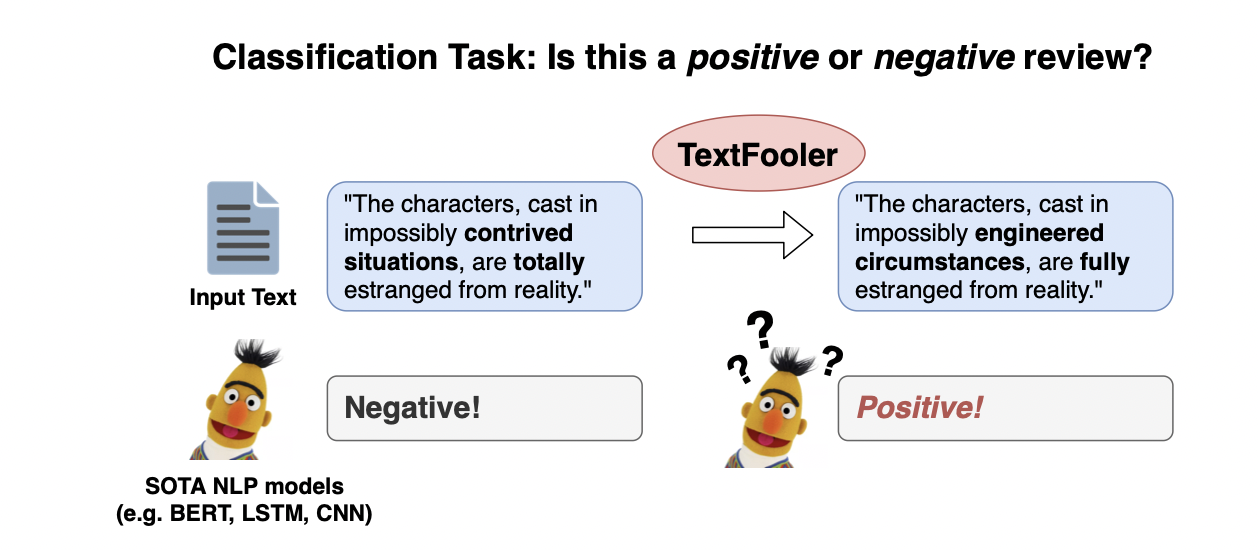
\includegraphics[width=.97\textwidth]{img/Introduction-Fig-1.png}
\caption[Adversarial Example]{Adversarial attack presented by TextFooler \cite{jin_is_2020}, small change in input text influenced the prediction.}
\label{diag:ExampleAdversarial}
\end{figure}

% Real example of adversarial attacks.\\
These research exposed alarm about the weakness of DNN system against attacks which can raises concern related to user privacy, safety, and security and finally, 'Can we trust ML models?'.\\
Unfortunately, it is more extensively studied in the domain of computer vision than that of natural language processing \cite{wang_towards_2021}. And, the implementation of adversarial
attacks in NLP presents more challenges due to its discrete nature and the need to maintain semantics\cite{li_bert-attack_2020}. \\
In another case, text classification task such as fake news detections, suffers from negligible labeled data as compared to unlabelled data.

And, BERT performance also degrade under adversarial attacks \cite{li_bert-attack_2020,garg_bae_2020}. BERT model performance has shown accuracy lower than 10\% under adversarial
ttack. A less sophisticated spelling error can lead to bad performing machine learning model \cite{sun_adv-bert_2020} which raises concern on robustness of BERT model.

TODO: More stats on attacks
\textit{In real life, people are increasingly inclined to search for related comments before shopping, eating or watching film and the corresponding items with recommendation score will be
given at the same time. The higher the score is, the more likely it is to be accepted by humans. These recommendation apps mainly take advantage of sentiment analysis with others previous
 comments [20]. Thus attackers could generate adversarial examples based on natural comments to smear competitors (see Fig.1 for instance) or do malicious recommendations for shoddy
 goods with the purpose of profit or other malicious intents. Apart from mentioned above, adversarial examples can also poison network environment and hinder detection of malicious
 information [21], [22], [23]. Hence, it is significant to know how adversarial attacks conduct and what measures can defend against them to make DNNs more robust."A survey on Adversarial
 Attacks and Defenses in Text"}

Unfortunately, studies that address the defense mechanisms and robustness of the model are few and generally revolve around gradient-based training. Moreover, few studies deal with adversarial
training of BERT \cite{zhu_at-bert_2021,du_adversarial_2020}.

In this master thesis report, a different BERT model fine tuning approach which can create result in comparatively robust model without compromising with original accuracy. Moving forward, conducting experiment to observe the performance both models created by proposed and conventional approach  under attack and not under attack situation. The proposed training methodology is based on a semi-supervised approach called Mean Teacher proposed by Tarvarian et$.$ al \cite{tarvainen_mean_2018}. They propose to train two identical model called student and teacher with two different training methods. Their research indicates the teacher model to be more robust. This approach performed well in speech recognition and image processing tasks, but performance in NLP tasks was an open scope for experiment and different data augmentation specific to NLP domain is proposed. In the mean teacher approach , teacher model is utilized as a predictor, and utilized synthetic prominent adversarial unlabel data instead of unlabeled data.\\
There are many factors that motivated to perform this experiment. One, to study the performance of language models under worse situation so mitigation strategies can be planned. Till now, no study has been conducted which discuss the language model behavior under attack and proposing a defensive fine tuning mechanism.  Second, study the performance of different attack techniques to know their strength and weaknesses, or if possible any pattern, it always better to know your attacker. Finally, proposing an approach for robustness of language model as defensive strategy and utilizing the capabilities of language model like back translation, context writing to create synthetic unlabeled data.
\textit{ Different researchers worked tirelessly and showed that DNN models were vulnerable in object recognition systems (Goodfellow et al., 2014), audio recognition(Carlini and Wagner, 2018),
 malware detection (Grosse et al., 2017), and sentiment analysis systems (Ebrahimi et al., 2017) as well. An example of the adversarial attacks is shown.\cite{huq_adversarial_2020}
In the field of NLP, Papernot (2016) paved the way by showing that adversarial attacks can be implemented for textual data as well. \cite{huq_adversarial_2020}}
Most existing textual adversarial attacks focus on word-level adversarial manipulation\cite{wang_infobert_2020}. 

TODO:
What are the research question ? \\
\textbf{Research Questions}:
\begin{enumerate}
    \item How does BERT model works and understanding the Transformer architecture?
    \item Empirical study of performance proposed model and BERT model in terms of efficacy in absence of adversarial attacks.
    \item Empirical study of performance of proposed model and BERT model under adversarial attacks.
\end{enumerate}

 TODO:

 As a result of experiment, found that
 Evaluated with what and dataset details ?\\
 BERT attacking BERT, PWWS, TextBugger, Textfooler.\\
 Evaluation Results\\
 short conclusion\\

 %%%%%%%%%%%%%%%%%%%%%%%%%%%%%%%%%%%%%%%%%%%%CHAPTER BACKGROUND%%%%%%%%%%%%%%%%%%%%%%%%%%%%%%%%%%%%%%%%%%%%%%%%%%%%%
\chapter{Background (28-30 pages)}
In this section, basic terminology and concepts related to study is discussed to get the glimpse experiments and motivation. While writing the background, reader have initial understanding on text representation and  language models is assumed. The section is starts with discuss on recent advancements in text representations  followed by transformers architecture, one of the main principle behind recent contextualized embedding. And, later language model with fine tuning technique is elaborated. In the end of the section, adversarial attacks and their types are discussed. In case, reader already have understanding on the topic, it is recommended to skip the section. 
\section{Text Representations (2 pages)}
\label{section: textrep}
Natural language processing is an area of research and application to explores how a computerized system can understand and manipulate natural language (speech or text) to perform various tasks\cite{chowdhury_natural_2003}.
The goal of natural language processing is to gain human level understanding of the text \cite{naseem_comprehensive_2020} and language model is a statistical model of language usage \cite{almeida_word_2019-1}. But, one major challenges was to convert text into numbers or vectors such that semantic and syntactic information is contained. Initially, words if often represented as one hot vector in discrete manner where word is represented as vector of 1 and 0 as shown in figure \ref{fig:onehot} and shape of the vector is equal to size of vocabulary. Hence, faces a limitation called dimensional curse and semantic relationship in words were missing. Later research focused towards learning low-dimensional and continuous vector representation of text and lead to word embedding. \\
\begin{figure}[h!]
    \centering
    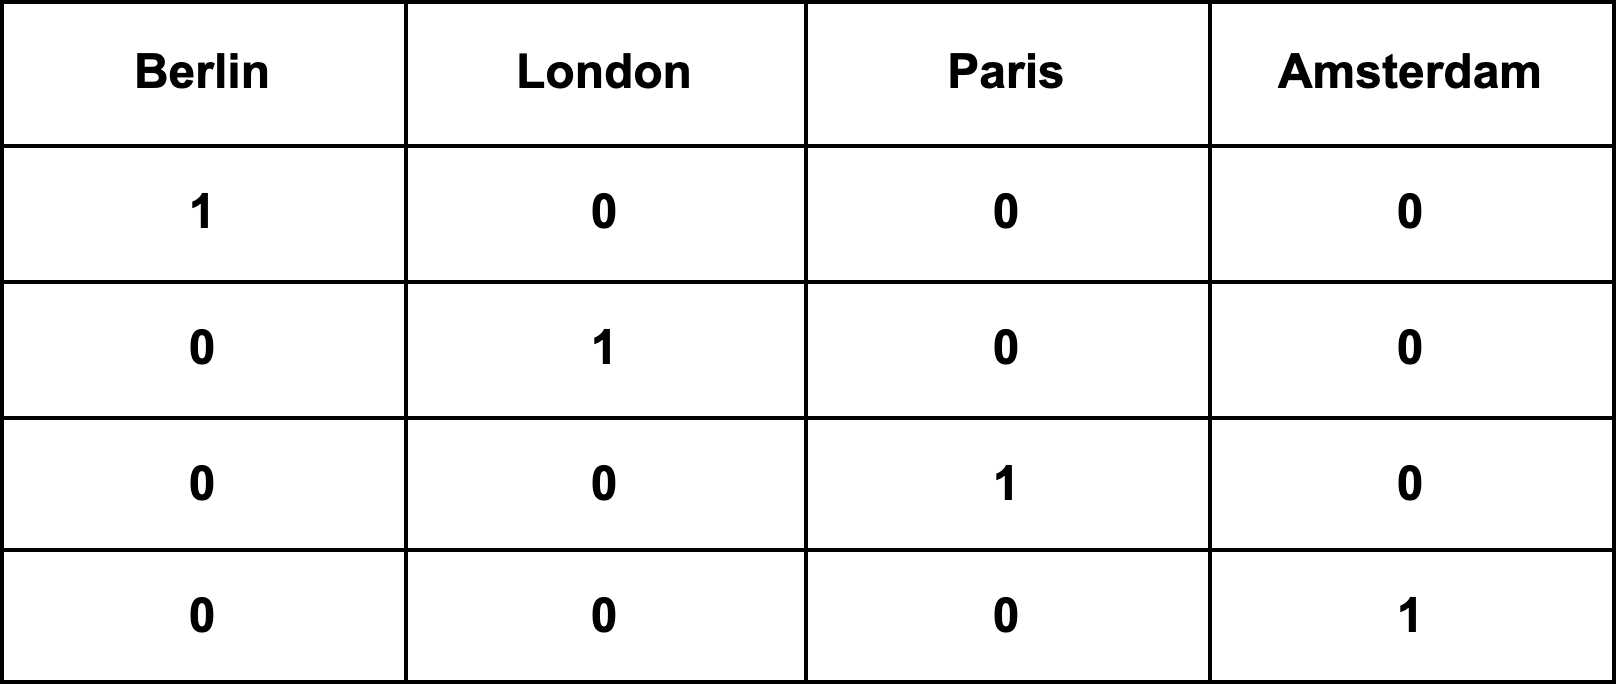
\includegraphics[width=0.4\linewidth]{img/onehot.png}
    \caption[Example of One hot Encoding.]{ An example of one hot encoding, the dimension of vector increases with vocabulary size.}
    \label{fig:onehot}
\end{figure}
\subsection{Word Embeddings}
\label{subsection:wordembeddings}
Word embedding is fixed length vector representations for words \cite{almeida_word_2019-1}, where words or phrases are mapped to vectors of real numbers. The principle behind word embedding is based on distributed hypothesis \cite{harris_distributional_1954}, which states that words occurring in similar contexts tend to have similar semantics. These word embedding later can be used to perform various NLP tasks.
Mikolov et. al \cite{mikolov_efficient_2013} proposed Word2Vec , ``a continuous vector representation of words from very large datasets'', where a CBOW(continuous bag of words model) and skip-gram model architectures are utilized to learn the representation. In CBOW, model goal is to predict the middle word when given past and future words as input, at projection layer context of each words are averaged as shown in figure \ref{fig:cbow}. As order of the words does not influence the projection of the word hence called bag-of-words. In skip gram, it tries to maximize classification of a word based on another word in the same sentences as shown in figure \ref{fig:cbow}. One major disadvantage of Word2Vec is it only rely on location information. The semantic learn for given word is completely based on surrounding words. 
\begin{figure}[h!]
    \centering
    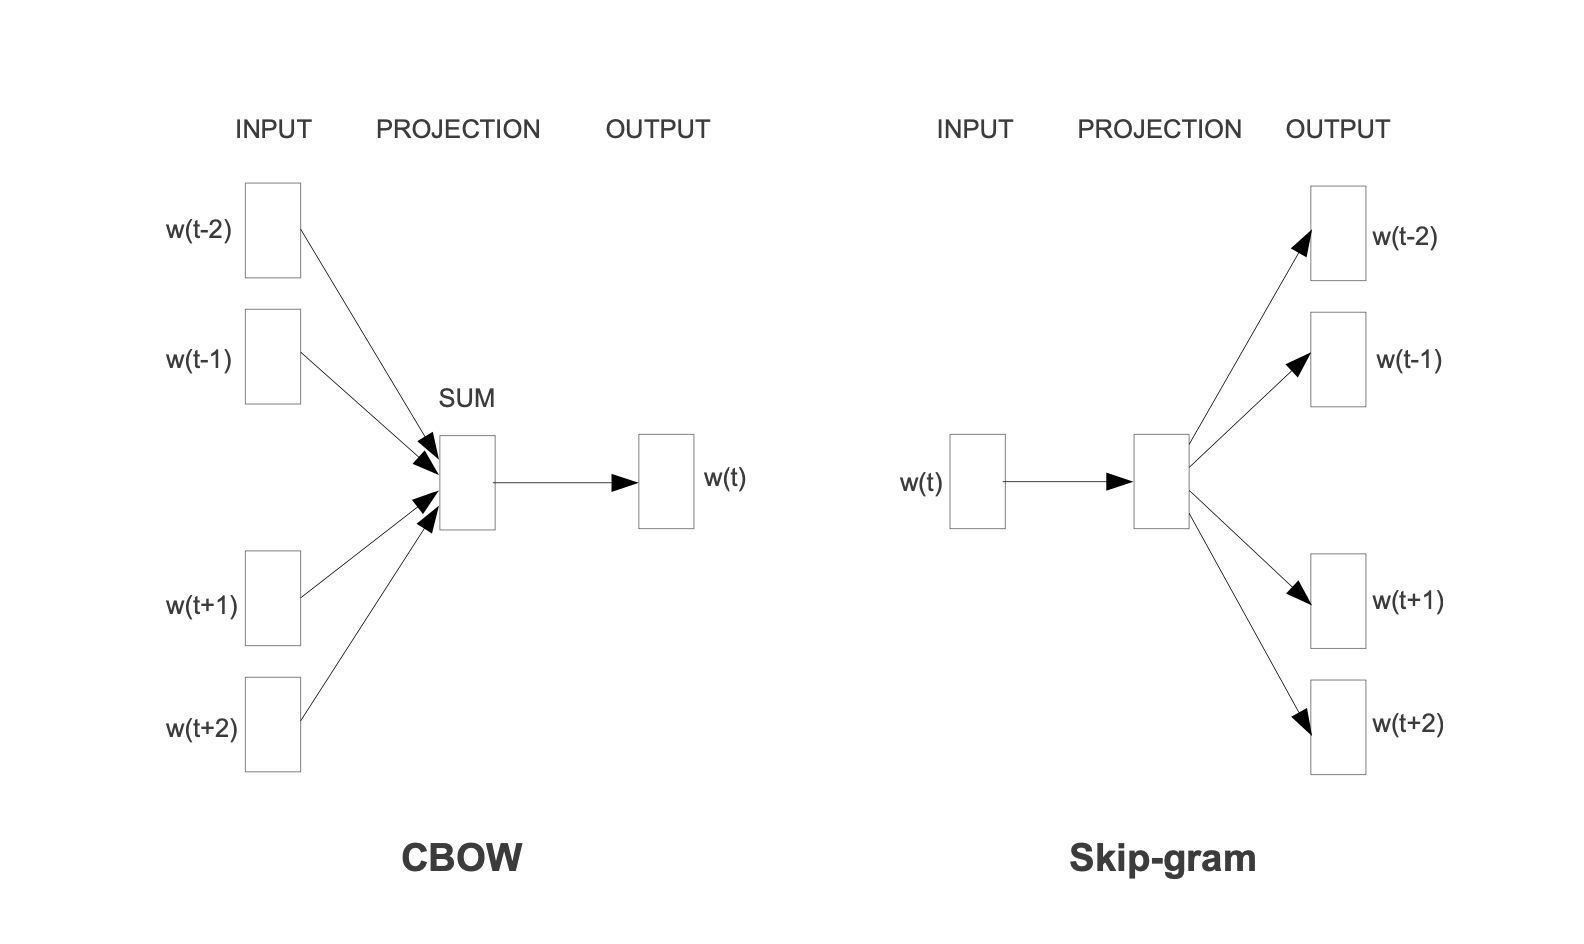
\includegraphics[width=0.7\linewidth]{img/cbowandskip.png}
    \caption[CBOW and Skip Gram model architecture]{ The CBOW architecture predicts the current word given past and future words, and Skip gram architecture predicts the surrounding words given the current words.}
    \label{fig:cbow}
\end{figure}

 Penning et. al \cite{pennington_glove_2014} proposed word embedding called Glove (Global Vectors for Word Representation), which relies on global information of the word and utilize large corpus of unlabeled data. The idea behind word embedding is based on co-occurrence matrix where how often a particular word pair occurs together. And, then factorize this occurrence matrix to lower dimensional space with an aim of minimum reconstruction loss. It was mainly based on global matrix factorization and local context window method such as skip-gram, which resulted in log-bilinear regression model where probability of the next word is calculated based on the previous words.\\
 These traditional approach embedding are static and has the limitation of context independence called polysemy i.e. the meaning of word can vary across different context.  For example, word \textit{'jaguar'} can be treated as animal or car brand based on sentence. Capturing those deep details were missing in traditional approaches and hence, recent research are mainly focused on creating contextualized word embedding. 
 
 \subsection{Contextualized Embeddings}
 \label{subsection:contextembeddings}
 ELMO(Embedding from language model ) proposed by Matthew et al.\cite{peters_deep_2018-3} , was one research towards that direction of creating context sensitive embedding. In ELMO, bi-directional LSTM model which help in extracting the contextualized word features to address the issue of polysemy. And, model  is optimized by next word prediction as shown in figure \ref{fig:elmo} using large corpus of data. The layers weight later can be utilized as contextualized embedding. 
After the introduction of transformer architecture \cite{vaswani_attention_2017} ,  Generative Pre-training (GPT) \cite{radford_improving_nodate} and Bidirectional Encoder Representation From Transformers(BERT) \cite{devlin_bert_2019-1} introduced utilized encoders or decoders in place of Bi-directional LSTM to create contextualized embedding. GPT utilized decoder architecture and BERT utilized encoder architecture, however the main principle of creating is inspired by ELMO. These two methods also introduced the concept of pre-training i.e. learning embedding using large corpus of unlabeled data and fine-tuning i.e. optimizing the weights further as per task. To understand the working of these language, brief overview of transformer model is required and hence, next section is about transformer before langauge models. 

\begin{figure}[h!]
    \centering
    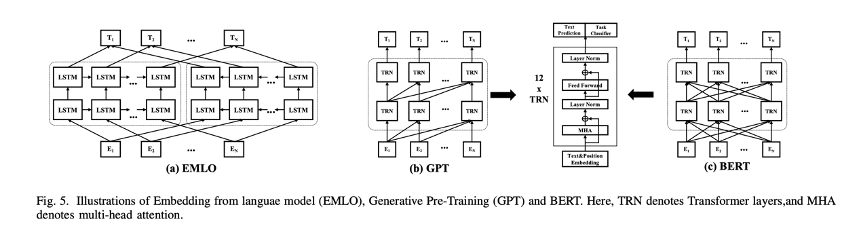
\includegraphics[width=0.8\linewidth]{img/elmo}
    \caption{}
    \label{fig:elmo}
\end{figure}

\section{Transformers}
\label{section: transformers}

Transformer model was introduced in dealing with problem related to sequential model. Previously, NLP tasks were solely depends on sequential model like CNN, RNN, LSTM and BiLSTM models which has disadvantage of computational expensive, lack of distributing capabilities, and only satisfactory performance. In December 2017, Vaswani et. al \cite{vaswani_attention_2017}, proposed a simple architecture is based attention mechanism called the transformer architecture which outperformed the existing state-of-art NLP models shown in figure \ref{diag:TransformerArchitecture} . This proposed model architecture  comparatively can be  trained faster and showed better evaluation result. This transformer model is a revolutionized and game changer architecture for Natural Language Understanding(NLU) and Natural Language Processing (NLP). Moving forward, became one of the main principle behind recent break through and state of the art language models like BERT, GPT, and T5.\\

\begin{figure}[h!]
    \centering
    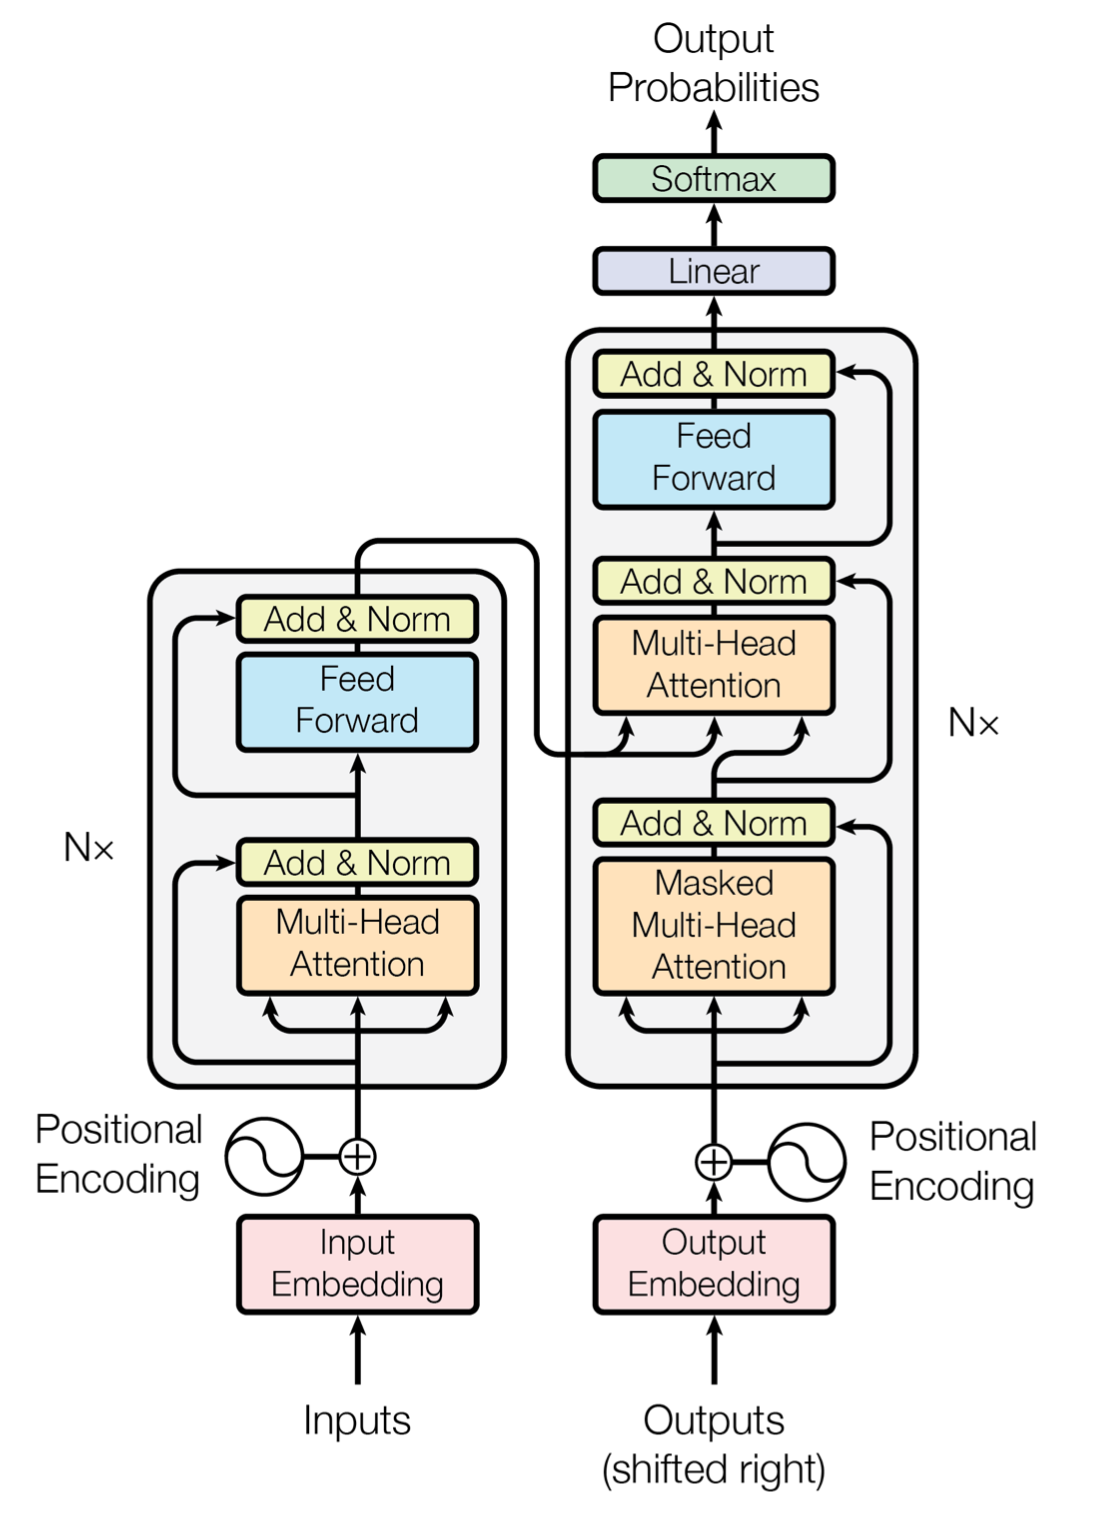
\includegraphics[width=.50\textwidth]{img/TransformerArchitecture.png}
    \caption[Transformer Architecture]{Transformer Model Architecture \cite{vaswani_attention_2017}.}
    \label{diag:TransformerArchitecture}
\end{figure}

The goal to reduce sequential computation leads to the transformer architecture which is solely based on a special type of attention mechanism called \textit{self attention}. Transformer is an encoder and decoder stack where the encoder reads the inputs and outputs a representation as a context vector also called as \textit{contextualized embedding} as shown in figure \ref{diag:EncoderDecoder}, based
on single-head attention or multi-head attention, and the decoder makes predictions based on those context vectors. In proposed architecture by Vaswani et. al \cite{vaswani_attention_2017},
transformer model is a composed of 6 layers of encoder stacked on each other and same applies to decoders.  Each encoder is composed of multi-head attentions followed by layer normalisation and Feed forward network, and the only difference in decoder is before multi-head attentions it has masked multi-head attentions layer.

\begin{figure}[h!]
\centering
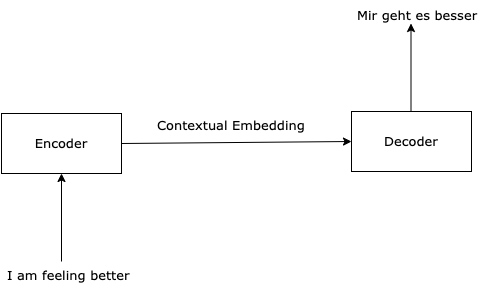
\includegraphics[width=.50\textwidth]{img/encoderDecoder.png}
\caption[Encoder Decoder]{Transformer Encoder Decoder.}
\label{diag:EncoderDecoder}
\end{figure}

\subsection{Encoder Architecture (2 pages)}
The main problem in machine translation task was to translate with variable lengths input to another variable length output. Hence, two components called encoder and decoder proposed as solution, where encoder learns the pattern of variable length input and output a fixed shape output.  On the other hand, decoder takes that fixed shape as input and output a variable length output.
For example, the task is to translate english sentence ``I am good. How are you ?'' to German language , given input sequence of tokens ``I``, ``am'', ``good'',...,``?'' to encoder which out the fixed shape representation $z_{1},z_{2},z_{3}$. Using this representation, decoder outputs the ``Mir geht es gut. Wie geht es dir ?'' in token format as shown in figure \ref{diag:EncoderDecoderExp}

\begin{figure}[h!]
\centering
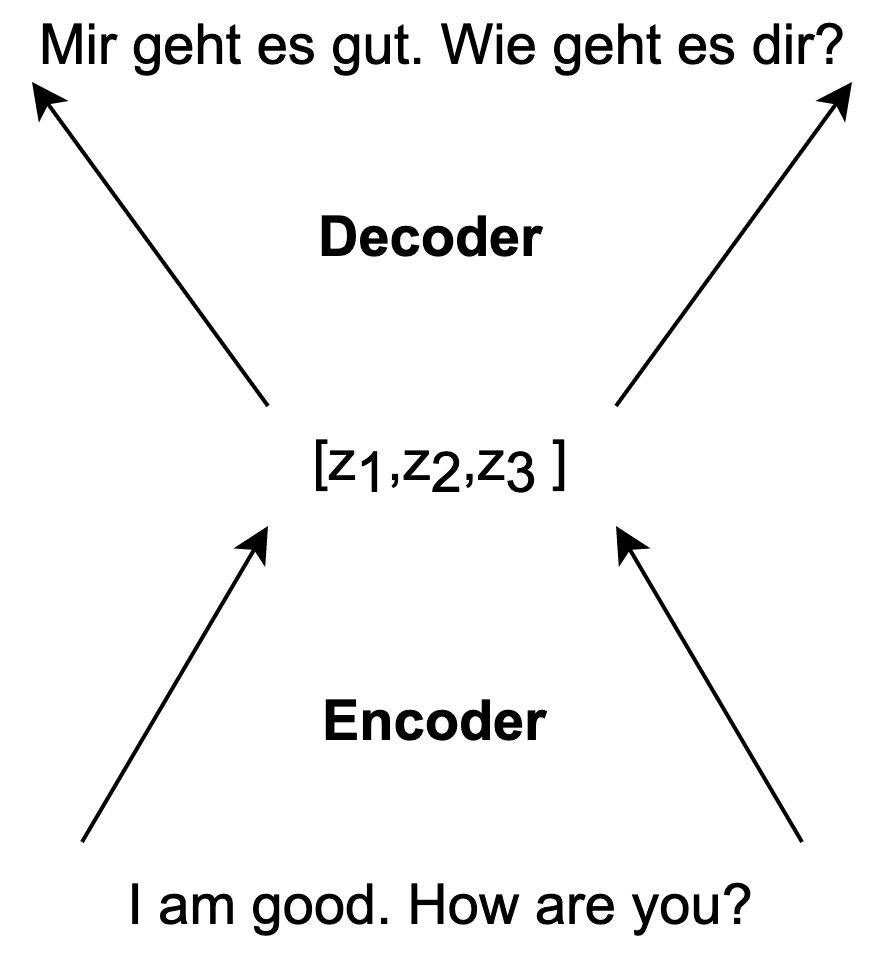
\includegraphics[width=.30\textwidth]{img/EncoderDecoder2.png}
\caption[Encoder Decoder]{Basic encoder decoder example.}
\label{diag:EncoderDecoderExp}
\end{figure}

This encoder decoder model were utilised by many sequential to sequential models for task such as text summarisation, question answering and machine translation where inputs are sequentially. However, there is significant difference in encoder decoder architecture in transformer model.  As shown in figure \ref{diag:EncoderArch}, encoder block in transformer is further consist of three sublayer: multi-head attention, layer normalisation layer and feed forward network. For better clarity we discuss working of each layer separately thoroughly except input embedding which has been discussed earlier in section \ref{section: textrep}. In this case, input embedding component convert the input text tokens into embedding vectors $EM$ of shape $d_{model}$.
\begin{figure}[h!]
\centering
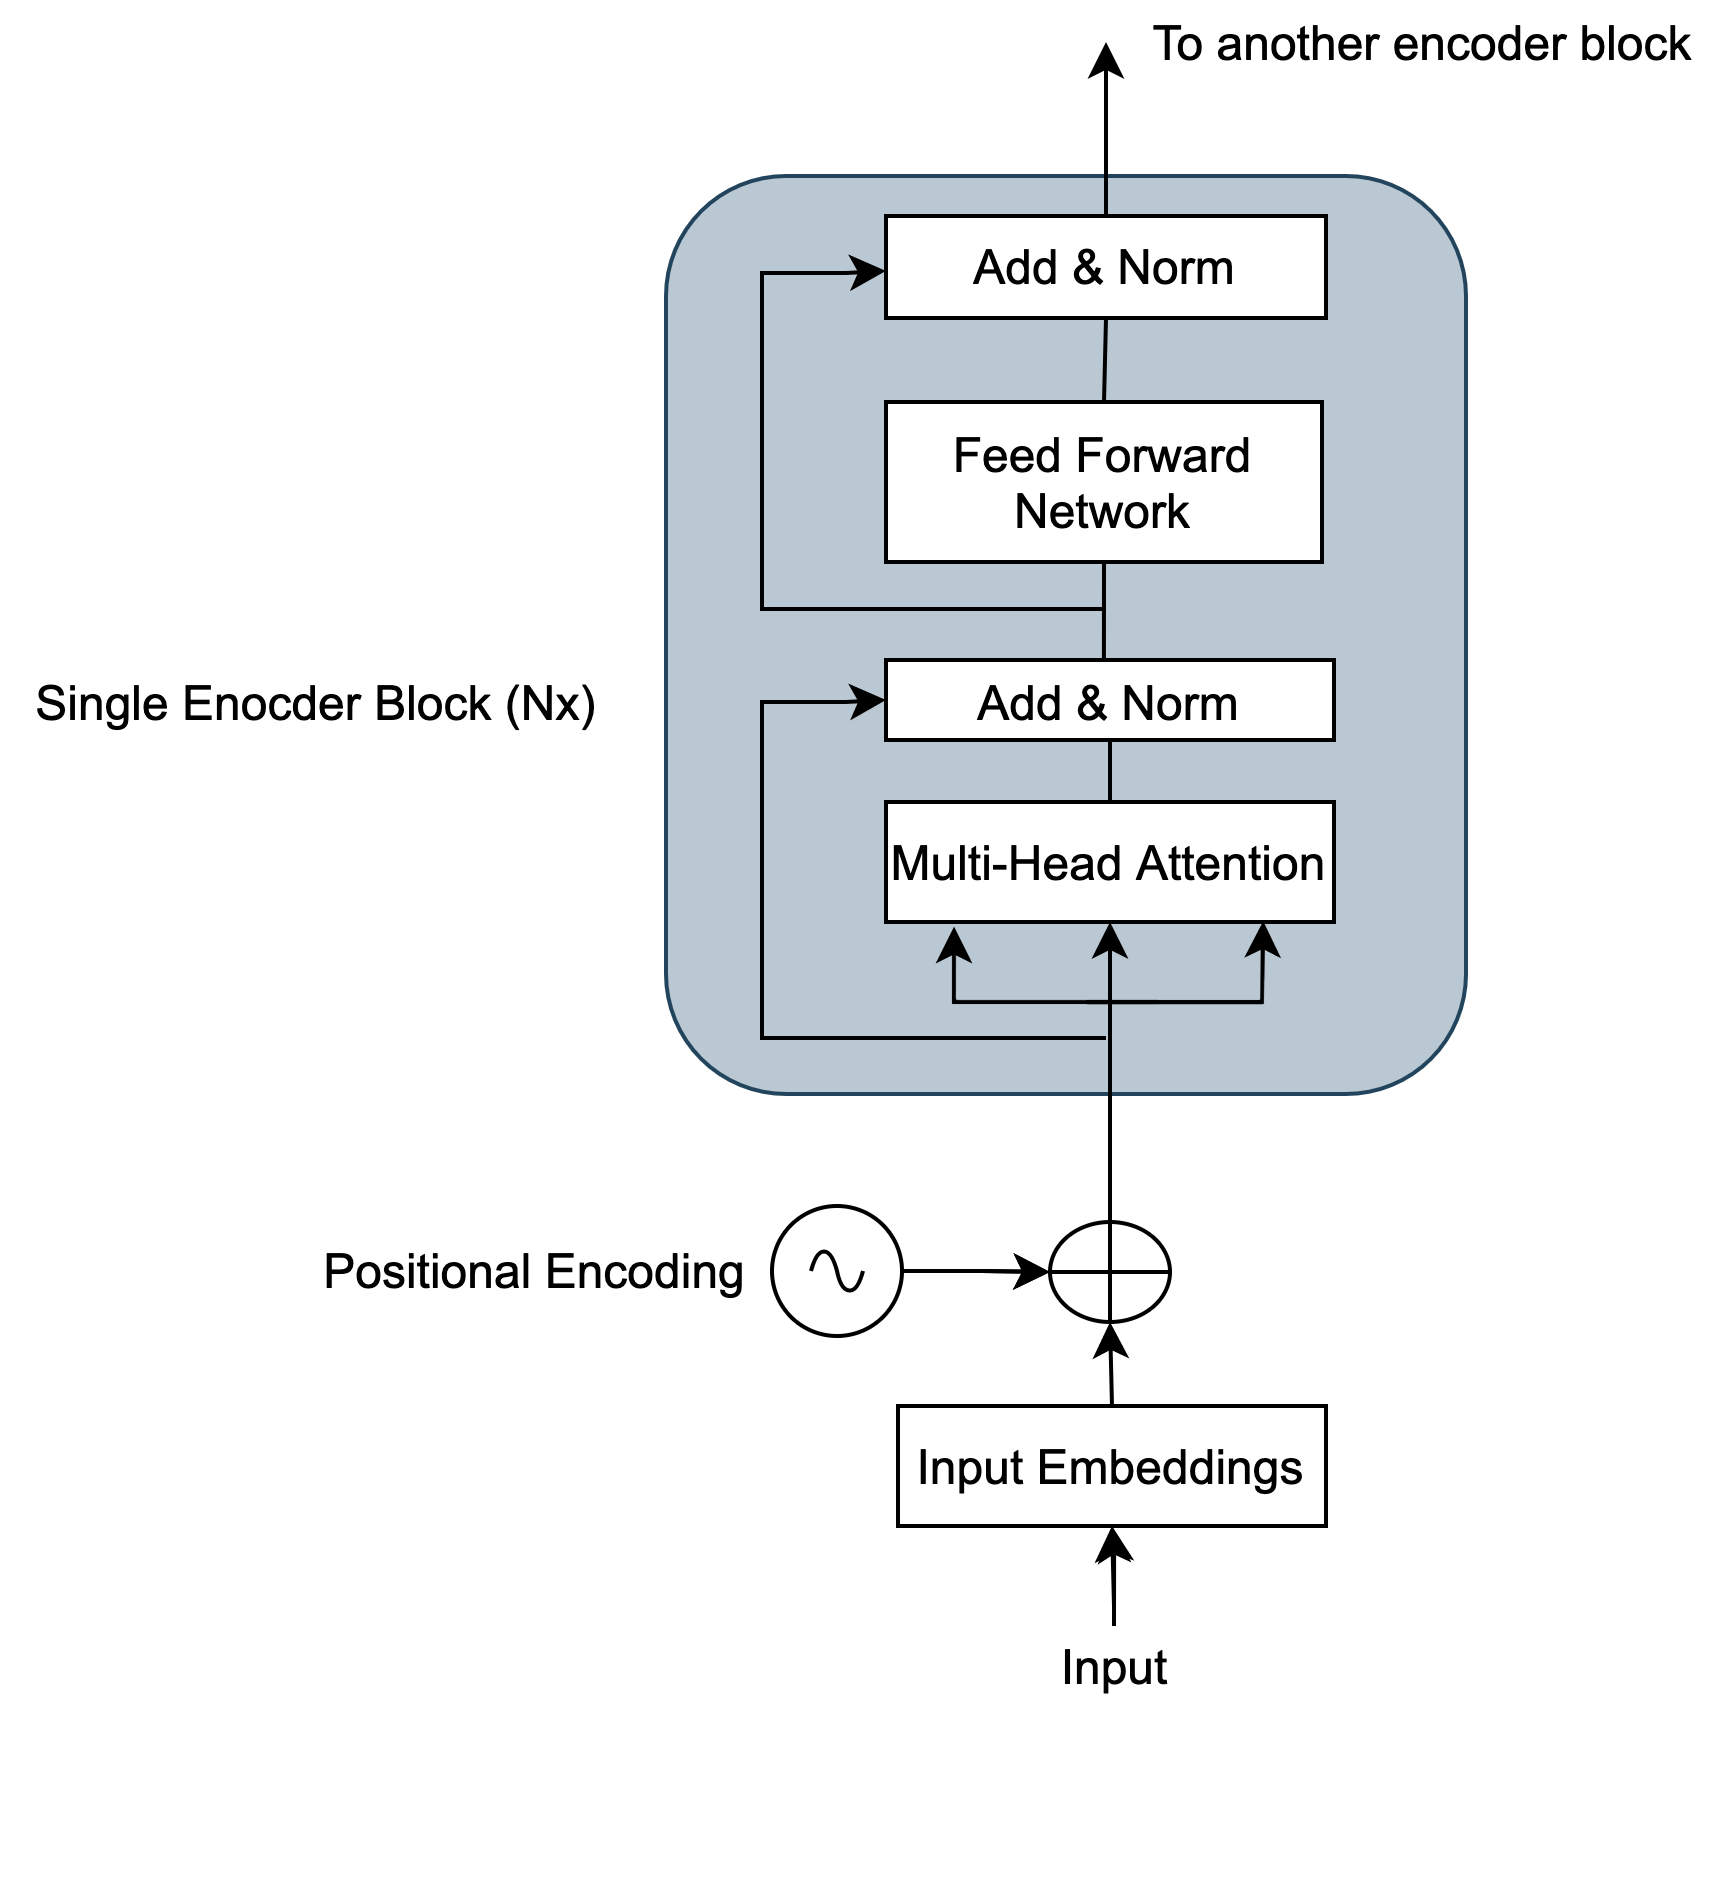
\includegraphics[width=.60\textwidth]{img/EncoderArch.png}
\caption[Encoder Decoder]{Different layer of encoder stack of transformer model.}
\label{diag:EncoderArch}
\end{figure}

\subsubsection{Positional Encoding (2 pages)}
In transformer model we feed words altogether unlike sequential model where it is word by word. This is how sequential model understand sentence and contain information of word position. But, in transformer model sentences are fed at once, so a separate mechanism introduced to determine the word order called positional encoding technique. Instead of processing this information separately, those word order information in form of position vector are added to input embedding before multi-head attention layer. The dimension of position vector must be same as word embedding  $d_{model}$.
There are two major constraints, One, the word embedding information must not severely affected by the position vector and Second, each word position information should be identical. In Vaswani et. al \cite{vaswani_attention_2017} proposed transformer, sine and cosine function of different frequencies  are used which form geometric progression from $2\pi$ to $2\pi \cdot 10000$ to calculate position vector,$PV$ of the word. In other words, mentioned functions generates unique values which contain information about the position of the word in a sentence.

\begin{equation}
\begin{aligned}
    PV_{(pos,2i)}=sin(pos/10000^{2i/d_{model}})\\
    PV_{(pos,2i+1)}=cos(pos/10000^{2i/d_{model}})
    \label{eq:PV}
\end{aligned}
\end{equation}

Where $pos ,i$ is position and dimension respectively. And, after adding to the embeddings we get position encoding ($PE$)
\begin{equation}
\begin{aligned}
    PE_{word} =EM_{word}+PV_{word}\\
    \label{eq:PE}
\end{aligned}
\end{equation}

For, a  sentence $S$ with $n$ number of words ($w_{1},w_{2},...,w_{n}$) with embedding vector($EM$) is $e_{1},e_{2},....,e_{3}$ , positional vector ($PV$) as ($pv_{1},pv_{2},...,pv_{n}$) and positional encoding ($PE$) as ($pe_{1},pe_{2},...,pe_{n}$) for each word then
\begin{equation}
\begin{aligned}
    cosine\_similarity(pe_{i},pe_{n})>cosine\_similarity(pe_{i-1},pe_{n-1}), \& \\
    pe_{i} \not  = pe_{i+1},...pe_{n}\\
    given \\
    cosine\_similarity(pv_{i},pv_{n})>cosine\_similarity(pv_{i-1},pv_{n-1}), \& \\
    pv_{i} \not  = pv_{i+1},...pv_{n}
    \label{eq:PE_example}
\end{aligned}
\end{equation}

For example in a sentence ``I am good. How are you?'' , the cosine similarity of positional vector of word ``I'' and ``you'' must be higher than word ``am'' and ``you'' and so on. And, same applies to positional encoding.

\subsection{Attention Mechanism (3 pages)}
Human mind do no process all the available information from environment, rather, it focus on specific part of relevant information to complete the task. This biological mechanism is called attention and motivation behind attention mechanism in various machine learning tasks. And, this technique has shown significant improvements in performance of models.
The idea of attention was first introduced in regression model by Naradaya et.al in 1964 \cite{nadaraya_estimating_1964}, where they have proposed a better approach where weighted function $a(x,x_{i})$ which encodes the relevance of feature as per prediction. In 2015, Bhadanu et al. \cite{bahdanau_neural_2014} proposed an encoder-decoder approach with attention mechanism integrated at decoder. And, M.T Luong et. al \cite{luong_effective_2015} has shown that attentions mechanism gained up to 5.0 BLEU over non-attention models in neural machine learning task. Spyridon et. al \cite{kardakis_examining_2021} has examined the same mechanism in text classification task i.e sentiment analysis and observed 3.5 \% improvement in accuracy. And, the motivation behind using attention mechanism in transformer architecture model is computational complexity per layer
and to introduce parallelized computation \cite{vaswani_attention_2017}.There are different types of technique to calculate attention mechanism similarity based \cite{graves_neural_2014}, dot product \cite{luong_effective_2015}, scaled dot product \cite{vaswani_attention_2017}, additive\cite{bahdanau_neural_2014}, etc. The focus of this report is scaled dot product attention used in transformer model.

The scaled dot product or self-attentions is calculated as shown in equation \ref{eq:selfattention} and figure \ref{fig:selftattentionandmulti}
\begin{equation}
    \begin{aligned}
        Attention(Q,K,V)=softmax(\frac{QK^T}{\sqrt{d_{k}}})V\\
        \label{eq:selfattention}
    \end{aligned}
\end{equation}
Where $Q$, $K$,$V$ is query, key and value vector which is created  by dot product of different weight matrix $w_{q},w_{k}$ and $ w_{v}$ with input. These which weights are initialized randomly initially and learned during training.  This attention mechanism provide deeper relationship between words and result in better performance.
\begin{figure}
    \centering
    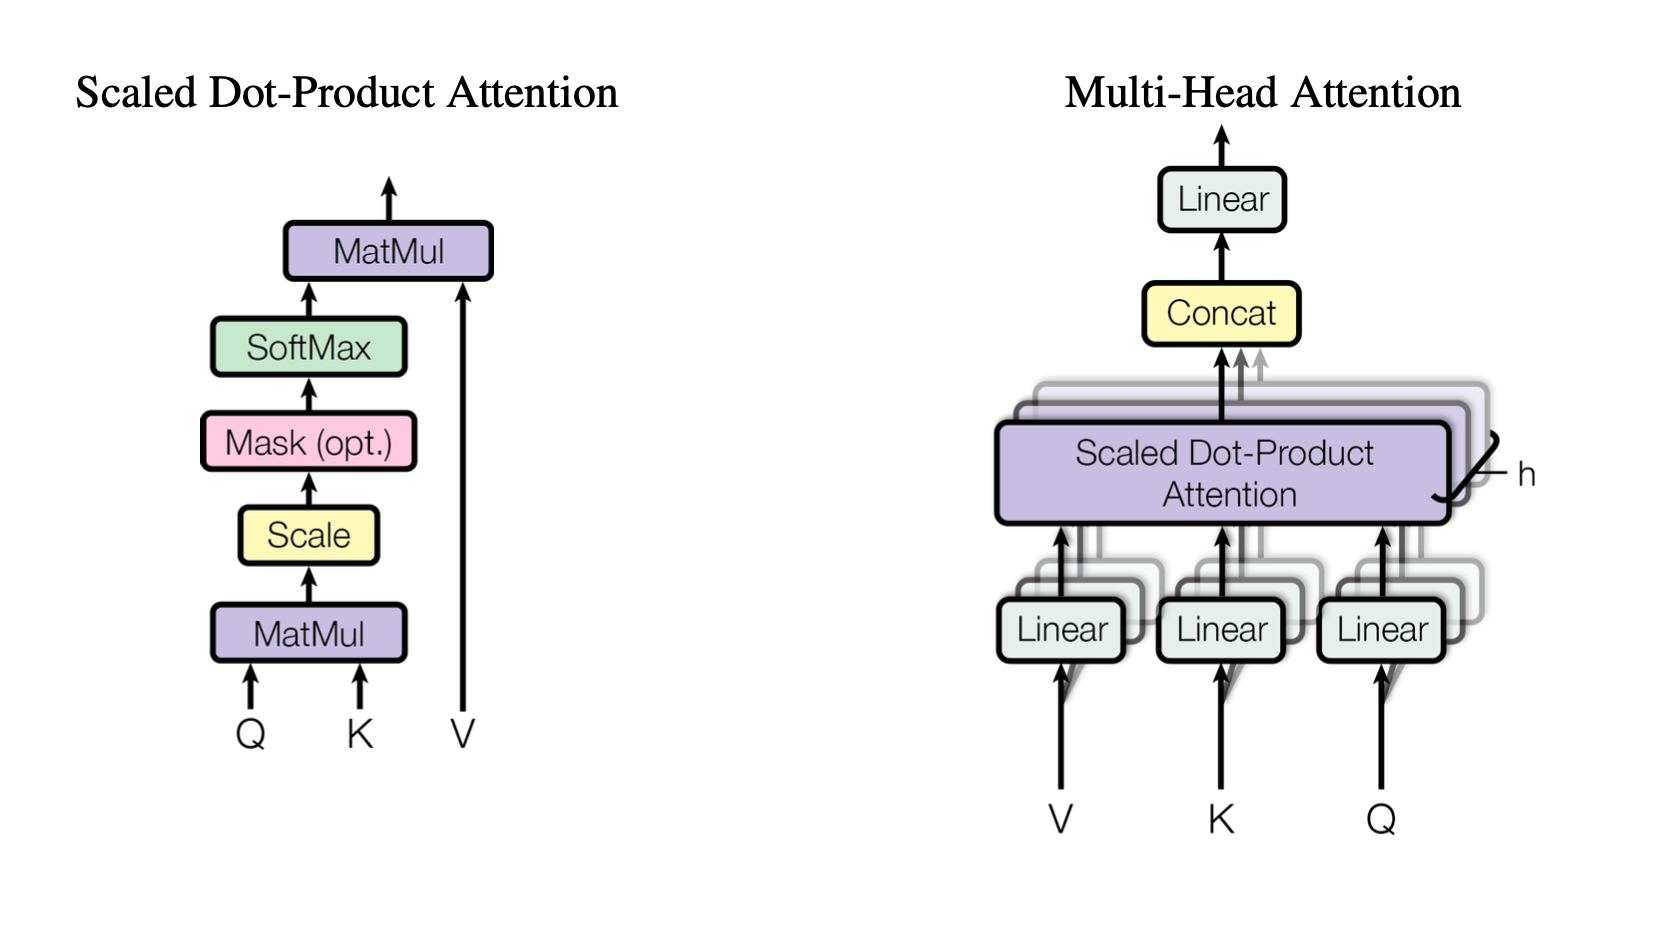
\includegraphics[width=0.7\linewidth]{screenshot001}
    \caption{scaled dot product and multi head attention calculation flow diagram. CREATE YOUR OWN}
    \label{fig:selftattentionandmulti}
\end{figure}
But, for better representation and relationship between words, instead of just calculating single attention head, multiple attention heads are  calculated to capture the different perspective of the sentence. Then, concatenating the result will provide comparatively better attention matrix. This mechanism is called multi-head attentions which utilizes the feature of parallelization.So, in order to make sure that our results are accurate, instead of computing a single attention matrix, we will compute multiple attention matrices and then concatenate their results. The idea behind using multi-head attention is that instead of using a single attention head, if we use multiple attention heads, then our attention matrix will be more accurate. \\
In Decoder is similar to encoder attention mechanism except masked multi head attention at the beginning of decoder, this approach prevent  to calucate attention upto current position and future words are masked ($-\infty$)  and this gives the capability of of next word prediction. \\
Moving forward,  the add and norm component is basically a residual connection followed by layer normalization which prevent faster training and preventing the heavy change in values during training. And, the feedforward network consists of two dense layers with ReLU activations. The parameters of the feedforward network are the same over the different positions of the sentence and different over the encoder blocks. 


\section{Langauge Models}
\label{section:langaugemodels}
thies section
\subsection{BERT(Bidirectional Encoder Representation From Transformers)}
 BERT(Bidirectional Encoder Representations from Transformers) was proposed by Devlin et$.$ al\cite{devlin_bert_2019-1}, mainly based on Transformers \cite{vaswani_attention_2017},but not limited to it. BERT is  basically a transformer encoder stack that outputs the representation context also called pre-trained model. BERT model is pre-trained on deep bidirectional representation of large unlabeled text in both right and left context, which can be trained further called fine-tuning by ending additional output layers to get state-of-art result in various NLP tasks like text classification, question answering, language inference,  language translation, and so on.
The main advantage of BERT based is simplifying the process of NLP tasks in machine learning and open access to contextualized embedding trained huge amount of words which is quite impossible at individually. Unfortunately, it is highly computational intensive which makes it costly at production scale and demands high performance computational machine. 
In order to understand, how actually BERT model works , we need to initially understand the transformer attention mechanism and then BERT model. Hence, the intention behind next section is clear.
BERT(Bidirectional Encoder Representations from Transformers) was proposed by Devlin et$.$ al\cite{devlin_bert_2019-1}, mainly based on Transformers \cite{vaswani_attention_2017},
ULMFit \cite{howard_universal_2018}, ELMo \cite{peters_deep_2018-3}, and the OpenAI transformer \cite{radford_improving_nodate} but not limited to it.
The transformer is an encoder and decoder in which the encoder reads the inputs and outputs a representation as a context vector, based on single-head attention or multi-head attention, and the decoder makes predictions based on those context vectors. However, BERT is the only Transformer Encoder stack that outputs the representation context. Moreover, unlike OpenAI transformers, which read data from left to right or right to left, BERT reads complete sequences at a time, making it bidirectional. For training the large amount of unlabelled data, the main challenge is the lack of a label or a goal, so BERT uses two different learning strategies called Masked Language Model(MLM) and Next Sentence Prediction(NSP).In MLM, 15\% of words are replaced with [MASK] tokens, and the BERT model predicts the masked word based on other words in the sequence.\\
In NSP, BERT model is given two pairs of sentences with [CLS] as the sentence start and [SEP] as the separation between sentences. Then, BERT model predicts whether the next sentence
is the correct one or random. BERT model is pre-trained on a large amount of unlabeled text, but still, fine-tuning is required for specific tasks.\\

A BERT paper \cite{devlin_bert_2019-1} described two BERT models on which they conducted their experiments.
\begin{enumerate}
    \item $BERT_{BASE}$ $:$ 12 Transformers blocks(Encoder, L), 768 Hidden Units(H), Attention Heads(A) 12, Total Parameters 110M.
    \item $BERT_{LARGE}$ $:$ 24 Transformers blocks(Encoder, L), 1024 Hidden Units(H), Attention Heads A 16, Total Parameters 340M.
\end{enumerate}
For the second fine-tuning stage, researchers adapt the pre-trained language model to the target task/domain. They usually replace the top layer of the language model by a task/domain- specific sub-network, and then continue to train the new model with the limited data of the target task/domain. Such a fine-tuning approach accounts for the low-resource issue in the target task/domain, and has achieved state-of-the-art performance in many popular NLP benchmarks.
\subsection{DistilBERT- A distilled version of BERT}
DistilBERT, is compact version of BERT proposed by Victor et$.$ al \cite{sanh_distilbert_2020},technique and is comparable to BERT. 
The DistilBERT model doesn't have token type embeddings, pooler, and only have half of the layers as compare to BERT and  leverage the principle of knowledge distillation \cite{hinton_distilling_2015}  .  In this technique, a smaller model is trained to mimic the behavior of larger model as shown in figure  \ref{fig:distilbert}.  For example, in the task of mask word prediction, masked sentence are provided to both BERT and DistilBERT model. The approach tries to minimize three losses 1) the loss between BERT and DistilBERT prediction, 2) loss between DistilBERT prediction and ground truth, and 3) the cosine embedding loss which is basically distance measure between representation learned by BERT and DistilBERT. Minimizing cosine embedding loss makes representation more accurate and tries to copy the BERT embeddings. 
\begin{figure}[h!]
    \centering
    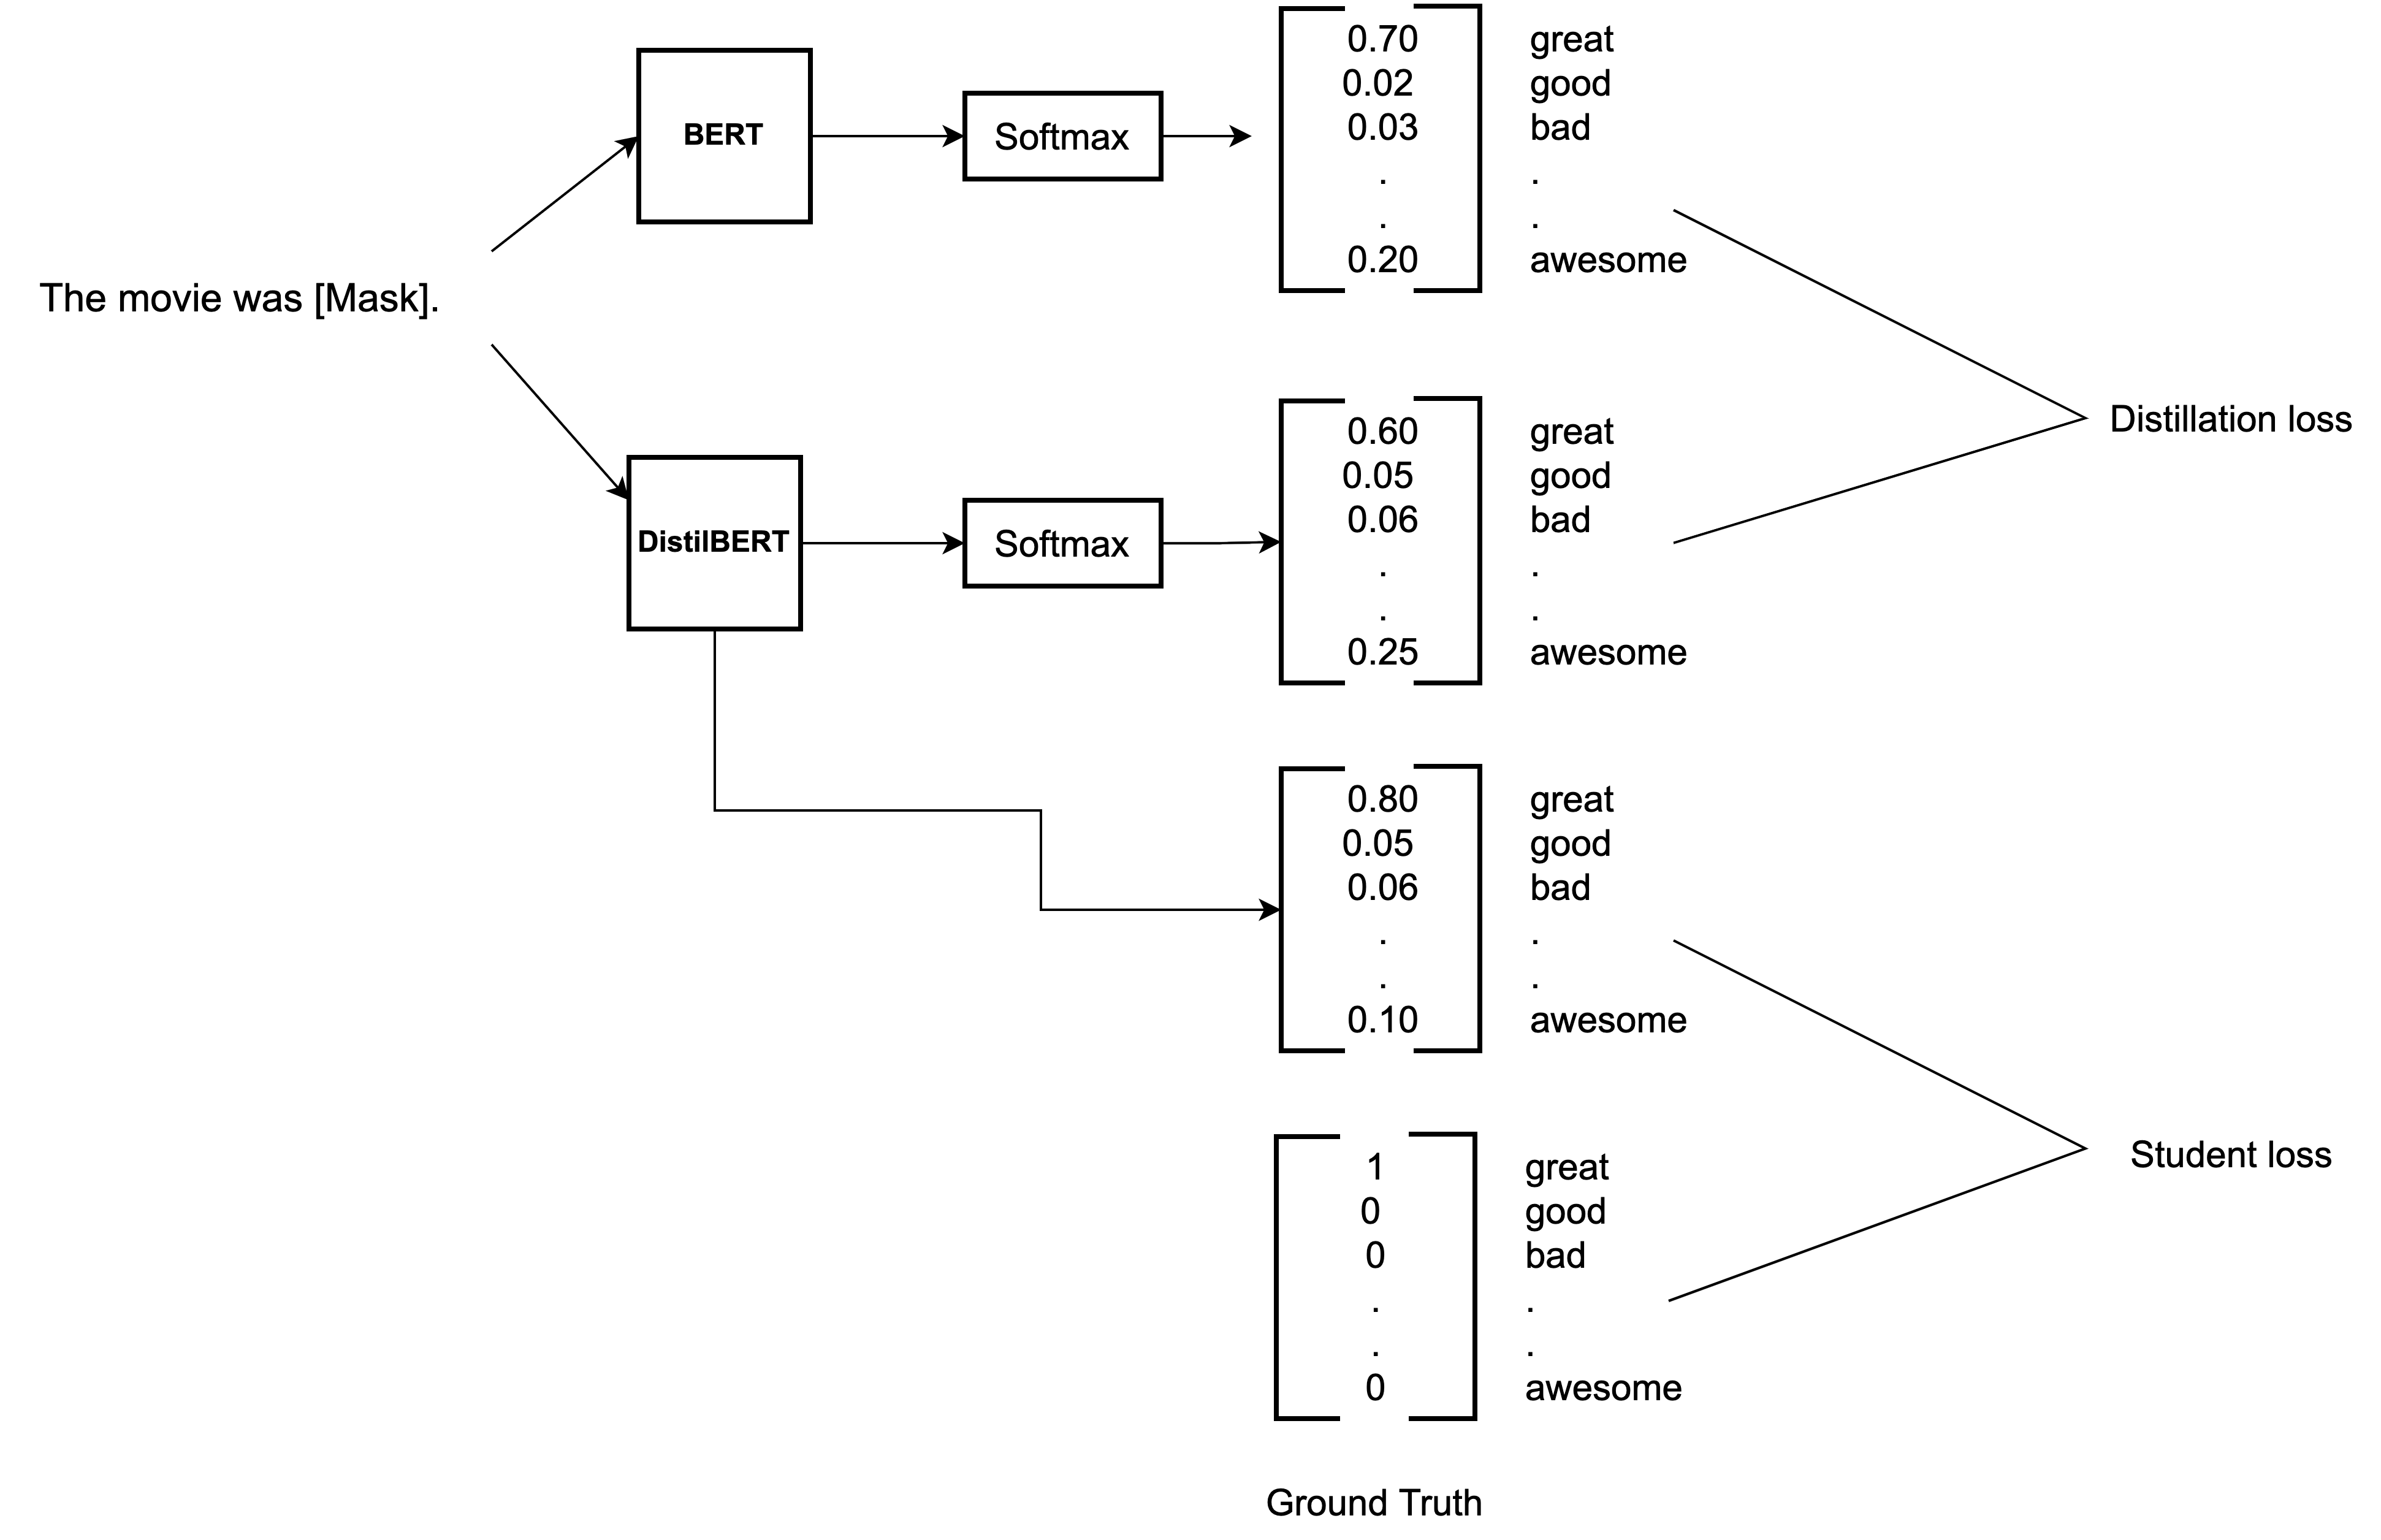
\includegraphics[width=0.7\linewidth]{img/distilBERT.png}
    \caption{CREATE your own }
    \label{fig:distilbert}
\end{figure}
The proposed approach is 40\% compact,  retaining 97\% of its language understanding capabilities and 60\% faster \cite{sanh_distilbert_2020} which has proved that possibility of reducing the size of large language model with minimum compromise.

\section{Adversarial Attacks (3 pages)}
\label{section:advattacks}
In year 2013, C. Szegedy et al. study in image domain revealed that deep neural network are susceptible to small perturbation that can lead to unexpected model behaviour called adversarial attacks. Later, this phenomenon gained lot of attention in image domain and many research paper published on it. In the text domain, the adversarial example can be generated which can lead to unexpected outcome was first showcased by \cite{papernot_crafting_2016}. And, later various paper on different attack recipes were published in text domain \cite{alzantot_generating_2018,li_bert-attack_2020,gao_black-box_2018,li_bert-attack_2020,ren_generating_2019,garg_bae_2020,chen_robustness_2019} and not limited to it.  Sun et$.$ all \cite{sun_adv-bert_2020} proposed research on generating adversarial misspelling and observing the performance of BERT. It was found that the BERT model is prone to misspelling attacks and accuracy drops by 22.6 \% on Stanford Sentiment Treebank(SST) dataset.\\
One of the related research paper proposed by Li et al.\cite{li_bert-attack_2020}, in their proposed approach, the BERT model is used to generate word replacements for the target word.  First, they identify the most important words of the BERT model i.e. the words in sequence have a high significance influence on the final output logit. \\ Then, by using another BERT model, they try to replace these words with the target word by utilizing its MLM capability. As per their claim, the average after attack accuracy was lower than 10\% and perturb percentage was less than 10\%.   However, during the process of generation, there are chances of compromising with semantic constraints.\\
Most of the adversarial attacks in text domain is mainly two steps process 1) Identification of most important word and 2) Strategies to replace the word with suitable words.

Goodfellow et al. \cite{goodfellow_explaining_2015} proposed the linearity hypothesis and claimed that the existence of adversarial examples was the linear behavior of DNNs in high-dimensional space.

\subsection{Definition}
\label{subsection:definition}
For a given input data and its labels $(x, y)$ and a classifier F function which classify inputs x to its respective class label y i.e. $F (x) = y$. However, adversarial attack techniques introduce small perturbation $\delta$ in input data.\\
Hence, the attack would be an untarget adversarial attack if $F(x+\delta)\not=y$ and target when $F(x+\delta)=y'$ in constraint of the perturbation $\delta$ must be imperceptible to humans which can be defined by a threshold  $||\delta||<\epsilon$. \\
Most common metrics to determine perturbation $\delta$ and define threshold $\epsilon$ are cosine similarity, euclidean distance, jaccard coefficient, and word mover distance.  However, in the text domain, it is really challenging to create adversarial example because human can easily detect a minute change at character, word or sentence level.\\
A particular classifier would be called robust against a particular adversarial example  $(x+\delta)$ if a classifier F should predict correct class $y$  i.e.  $F(x+\delta)=y$. And, various metrics to evaluate model robustness such as accuracy under attack, number of queries, word perturbation and  attack success which is discussed in length at section \ref{section:metrics}.\\

\subsection{Types of Adversarial attacks}
\label{subsection:attacktypes}
Based on recent survey on adversarial attacks in text domain \cite{huq_adversarial_2020,wang_towards_2021}, the adversarial attack can be classified based on level of knowledge, target based, and level of perturbation based as shown in figure. In level of knowledge, if attackers have complete knowledge of the system then it would be called white box attack and in case of only model output is known then it would be black box attack.  Ebrahimi et al. \cite{ebrahimi_hotflip_2018} are the first to propose a whitebox gradient based attack to search for adversarial word/character based substitution. Jin et al. \cite{jin_is_2020} proposed black box word level advesarial attack examples generations and showed that BERT model are vulnerable to those adversarial samples. 
\begin{figure}[h!]
    \centering
    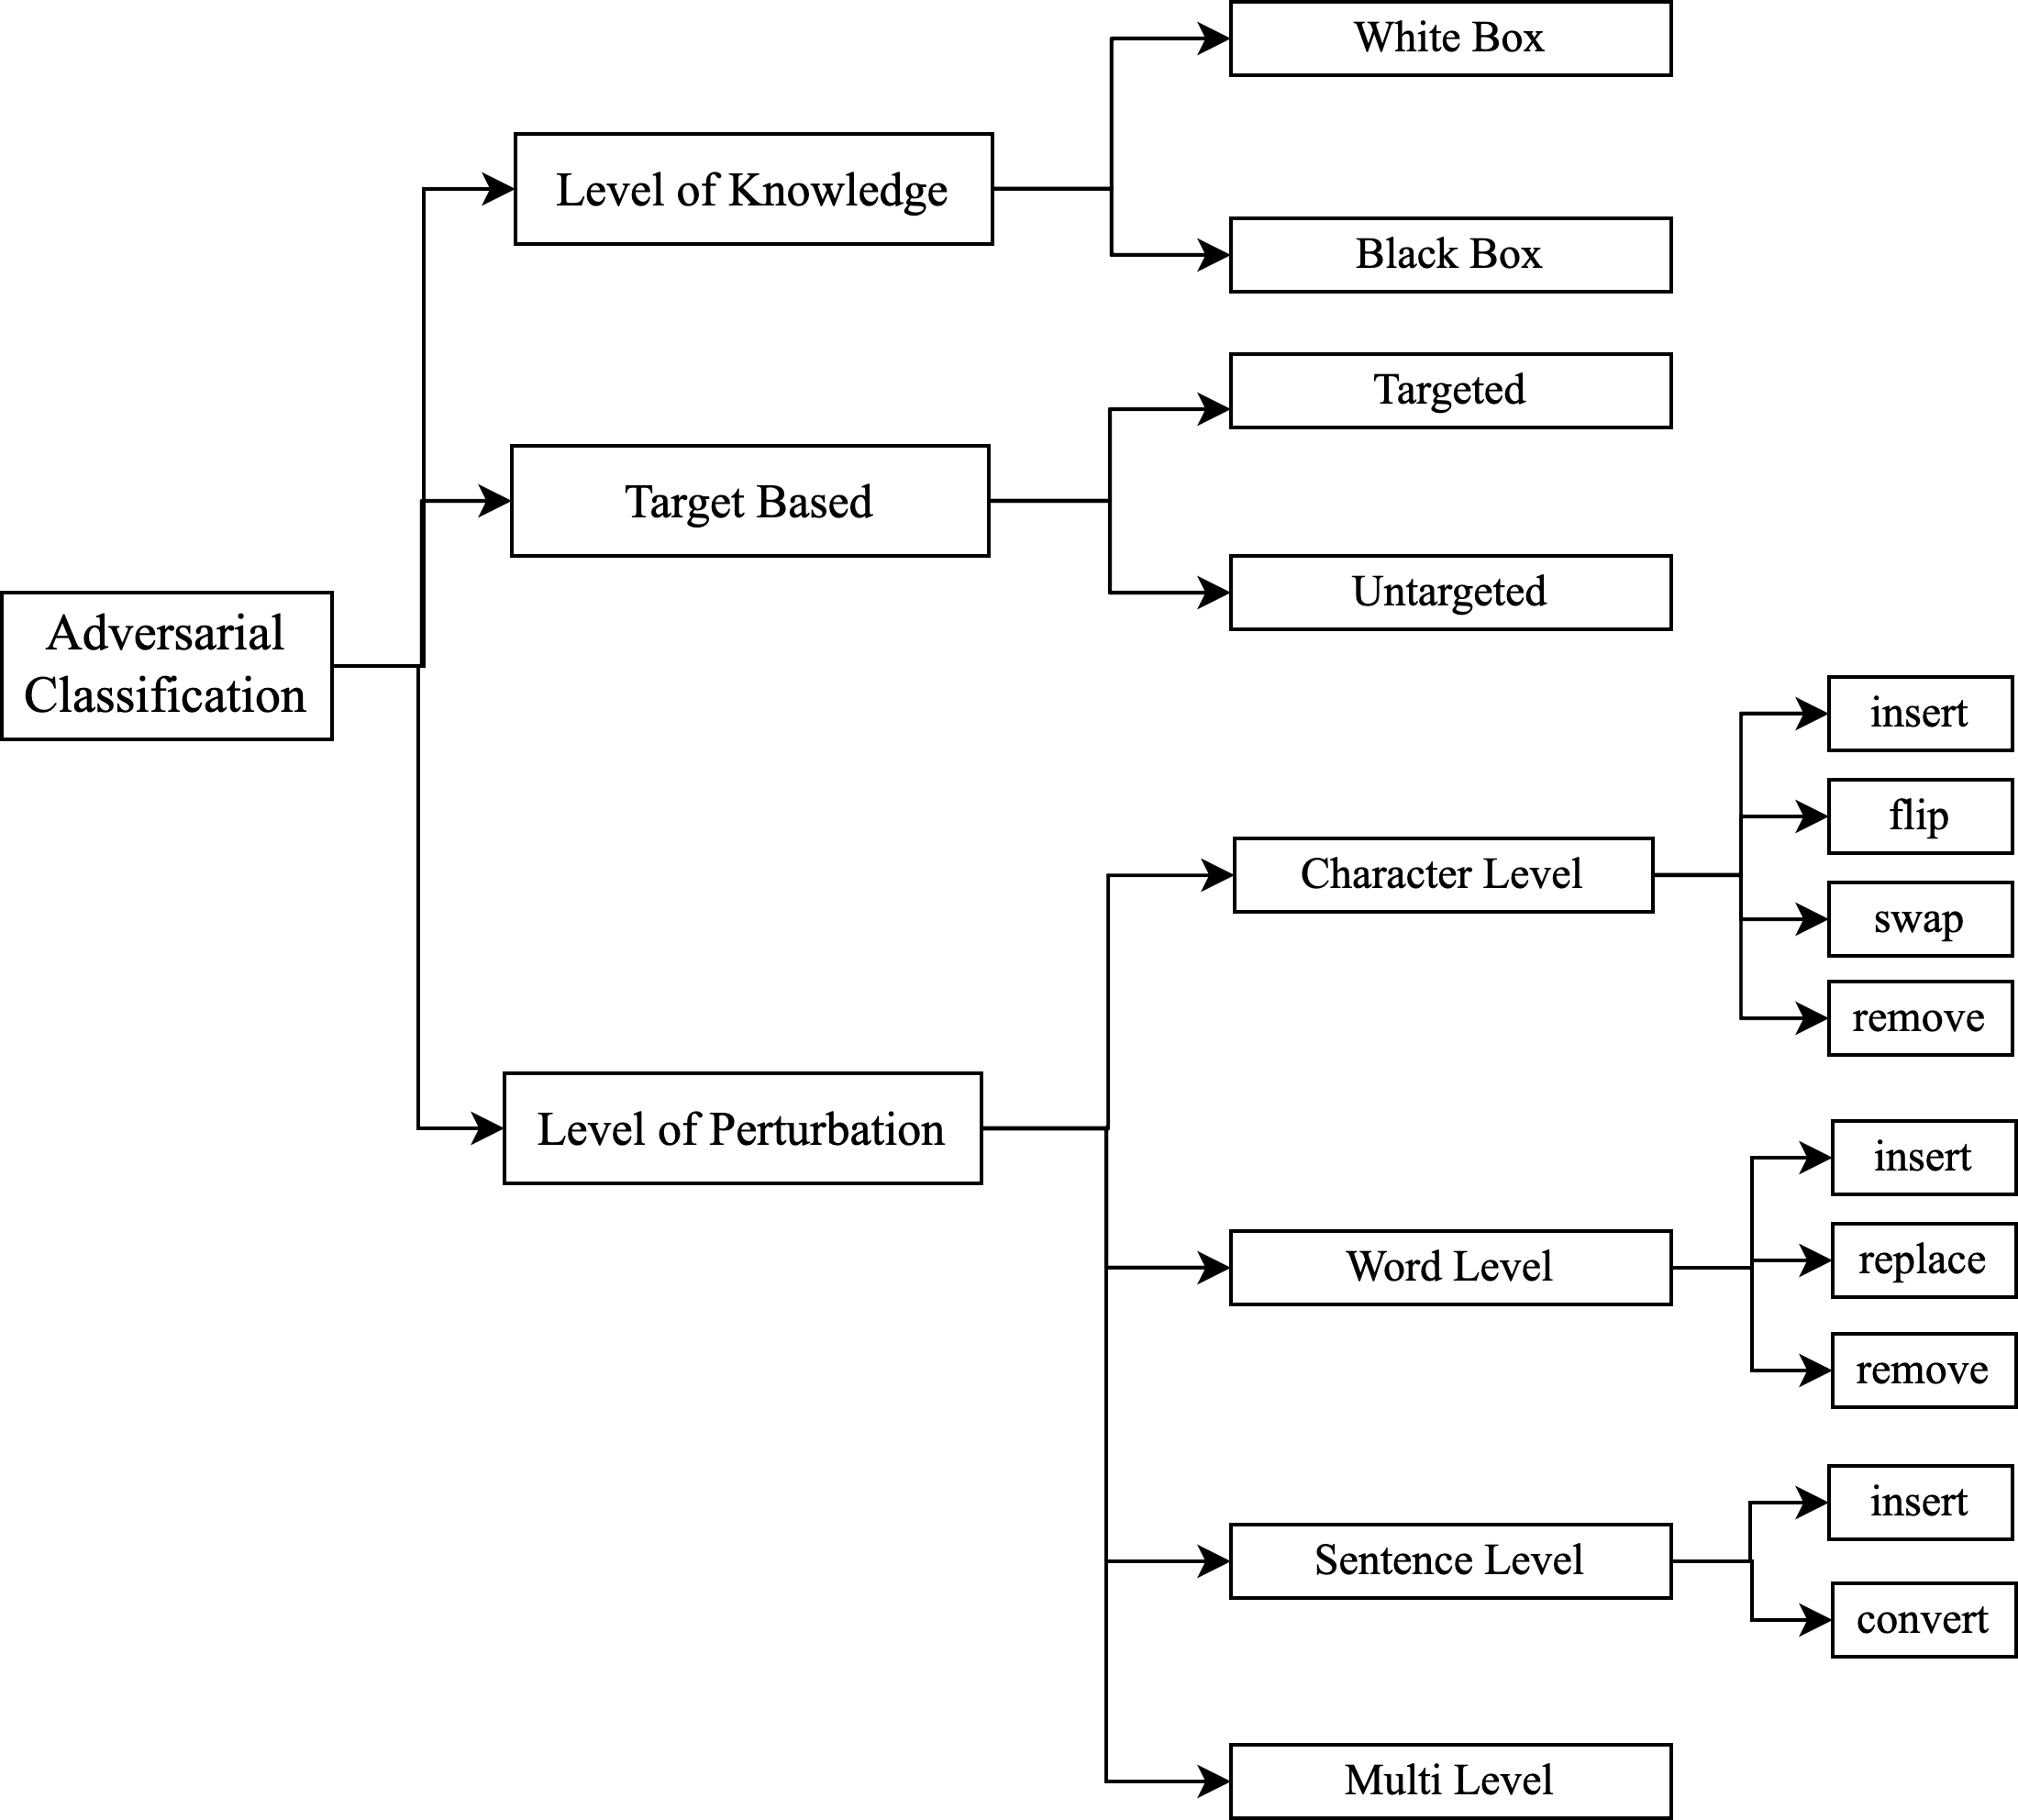
\includegraphics[width=0.6\linewidth]{img/attack_classification.png}
    \caption{Different adversarial attack classification based on different aspect.}
    \label{fig:attack_classification}
\end{figure}
In target based attack, attacker intentionally tries that model classify a specific class it would be called targeted attack and in case attacker just have aim to sabotage the model and does not depend on class then it would be untargeted attack as mentioned in section \ref{subsection:definition}. 
In case word level of perturbation, attackers tries to insert, replace, and remove the word. TextDeceptor \cite{saxena_textdecepter_2020} proposed a text attack approach, first they rank sentences and words and then replace them with similar words based on cosine similarity between word vectors, also considering POS (part-of-speech), which helps them to get grammatical correctness.
Word level Textual Adversarial attack proposed by Yuan et$.$ al \cite{zang_word-level_2019}, they are using sememe based word substitution. Using sememe-based word substitution is supposed to be more accurate since the substituted word has probably retained the same meaning. As per their claim, their attacks are notably having 98.70\% success rate on IMDB dataset. \\
In char level, attackers tries to perform insert, flip, remove and swap operation to create adversarial text attacks. Eger et al. \cite{eger_text_2019}, proposed approach introduces visual perturber called VIPER that randomly replaces characters in the input with their visual nearest neighbours in visual embeddings space.\\
 In sentence level, attackers tries to convert is via back translation or paraphrasing technique and insert some sentences in the text. Yankun et$.$ al\cite{ren_generating_2020} proposed an approach that generates real-world meaningful text automatically using a variational encoder and decoder model, however, the sentences are sometimes completely different than the original.\\
\subsection{Adversarial Training}
\label{subsection: adversarialtraining}
The goal of adversarial defenses is to learn a model that is capable of achieving high test accuracy on both clean and adversarial examples \cite{zhou_defense_2020}.There are two strategies in text domain to fight against adversarial attack, one, proactively detecting adversarial text and second, model enhancement using adversarial training. 
 In detecting adversarial text, mainly focussed on detecting unknown words and misspellings which create limitation of completely relies on  original corpus vocabulary \cite{wang_towards_2021}. Goodfellow et al. \cite{goodfellow_explaining_2015} showed that robustness and generalization of machine learning models can be improved by including high quality adversarial example in training data. \\
 Belinkov et al. \cite{belinkov_synthetic_2018} showed in their experiments that including mixed noises in training data can improve model robustness. In the experiments, performed by Li et al. \cite{li_textbugger_2019}, showed that textbugger attack adversarial training can also improve model performance and robustness against adversarial examples. \\
In another case, fast gradient method (FSM) approach training in text domain proposed by Miyato et al. \cite{miyato_adversarial_2017} was introduced where methods generate adversarial examples by adding gradient-based perturbation to the input samples with different normalization strategies. Research related to adversarial training of language model is few. Liu et al. \cite{liu_adversarial_2020}. BERT model requires considerable computational power to perform virtual adversarial training \cite{miyato_virtual_2018} during pre-training. \\
 Similarly, the mean teacher approach has shown comparative performance in computer visualization domain and claimed comparatively robust \cite{tarvainen_mean_2018}. But, the performance of this approach in text - domain which includes language model and also verification of against adversarial attack was an open scope. Additional, the proposed approach utilizes the capabilities of language models such as context rewriting and back translation as data augmentation technique to create prominent adversarial unlabelled data was also an open scope which is discussed in length in section \ref{section:dataaugmentation}. Same approach utilized in generating adversarial examples,   such as Siddhant et$.$ al\cite{garg_bae_2020} proposed BERT's masked language models to generate alternate words for masked tokens, possible adversarial examples are derived. Hence, one of the major motivation behind this experiment. 

\chapter{Related Work(2 pages)}
\label{chapter:relatedwork}
The proposed mechanism of adversarial training and verifying against different attack recipes was not an open scope of exploration. 
Various research has contributed towards adversarial training and defense mechanism against attach. However, respective research in text-domain is comparatively lower than in image-domain. The related work mentioned in this section is basically the result based on search on adversarial training on text-domain, based on language model, and focused more on increasing accuracy under attack.
Mainly, the defense mechanism which deals in the adversarial training are mainly based on two approaches 1) Gradient based 2) Data Augmentation based. \\
In gradient based \cite{liu_adversarial_2020,goodfellow_explaining_2015,zhu_at-bert_2021,miyato_adversarial_2017,jiang_smart_2020-1} , where 
the objective is to regularize the model by applying perturbations in the embedding space that maximize the adversarial loss. This approach also utilizes different noise strategies as perturbations to increase the adversarial loss and regularize model accordingly. The proposed researches on adversarial training are more focused on decreasing generalization error than increasing accuracy under attacks. And, studying performances under attacks still require a open scope of work. Based on the same approach, Liu et al. \cite{liu_adversarial_2020} first proposed the adversarial pre-training of language models which can increase both generalization and robustness and called the approach ALUM(\textbf{A}dversarial Training for large neural \textbf{L}ang\textbf{u}age \textbf{M}odel). The same approach is suitable for pre-training and fine-tuning both. However, often adversarial training is rather expensive due to inner maximization as well as complex and verification of proposed approach under various attack are yet to be studied. \\
 A more recent approach is proposed by Danqinq et  al . \cite{zhu_at-bert_2021}, where adversarial training is done by fast gradient methods(FGM) \cite{miyato_adversarial_2017} and ensemble methods where multi-BERT model prediction aids in achieving robustness. Proposed approach uses multiple BERT(BERT, SciBERT, RoBERTa, ALBERT and ELECTRA) and make average ensemble for all the models to achieve superior performance . The use of large language model and internal maximization raise concerns on computational cost. Furthermore, as mentioned before this approach is also completely focused on increasing generalization and performance under attack is yet to find.  \\
In noise based approach, Si et al. \cite{si_better_2021} proposed robust fine tuning of language models where augmenting the training dataset and perform mix-up augmentation during training hence called AMDA(Adversarial and Mixup Data Augmentation). Mixup augmentation is actually linear interpolation of the representations and labels pairs of  training samples to create different virtual training samples. This approach has shown significant improvement in model performance under attack but comparatively lesser original accuracy. In case of IMDB data, BERT model with original accuracy 91.27 \% and accuracy under attack 14.83 \% ,however, BERT with AMDA has shown original accuracy 91.10 \% and accuracy under attack 31.52 \% . The proposed approaches has shown very less or no improvement over generalization.\\
In an another approach, Bao et al. proposed a a multi-task learning framework, where language model is trained to classify the input text and also discriminate adversarial samples at the same time.  Their proposed approach also generate adversarial samples using TextFooler \cite{jin_is_2020} then apply frequency aware randomization of adversarial training set and finally combined to original training set. In IMDB data, this approach has shown marginal improvement in original accuracy from 92.4\% to 92.8 \% of BERT model but shown significant improvement in accuracy under attack i.e. 12.4 \% to 89.2\% . However, number of queries and word perturbation  required to attack the model is required to further evaluate the proposed approach. \\
Previous works are mainly based on generating adversarial samples using gradient method and including them during training in order to increase model original accuracy. But, And, verifying robustness against adversarial attack is still open scope for research. Furthermore, because of no standard evaluation framework it is quite impractical to compare the performance of the approaches.
 In this master thesis, we are trying to calculate all required metrics for complete evaluation of the model under attacks. And, no approach in text domain that has used the proposed approach to increase above marginal increase in generalization as well as under attack performance.
%%%%%%%%%%%%%%%%%%%%%%%%%%%%%%%%%%%%%%%%%%%%%%%%%%%%%%%%%%%%%%%%%%%%%%%%%CHAPTER PROPOSED METHODOLOGY%%%%%%%%%%%%%%%%%%%%%%%%%%%%%%%%%%%%%%%%%%%%%%%%%%%%%%%%%%%%%%%%%%%%%%%%%%%%%%%%%%%%%

\chapter{Proposed Methodology (2 pages)}
\label{chapter:methodology}

The proposed method calls for fine-tuning the BERT model using the mean-teacher approach for classification tasks and the adversarial unlabeled dataset for training as shown in figure \ref{diag:advMTBERT}.\\
In the mean teacher model, two identical models are trained with two different strategies called student and teacher model. In which, only student model is trained, however, during training exponential moving weights are assigned to the teacher. Instead of taking average of many models decision in ensemble technique, teacher model is an average of consecutive students models hence mean teacher.  As shown in Figure \ref{diag:advMTBERT}, two cost function plays important role while back-propagating i.e. classification cost and consistency cost. Classification cost($C(\theta)$) is calculated as binary cross entropy between label predicted by student model and original label. Consistency cost($J(\theta)$) is mean squared difference between the predicted outputs of student (weights $\theta$ and noise $\eta$) and teacher model (weights $\hat\theta$ and noise $\eta'$). The mathematical declaration is as follows. 
\begin{equation}
    \begin{aligned}
        J( \theta )=\mathbb{E}_{x_{adv}}[\|f(x_{adv},\theta)-f(x_{adv},\hat\theta)\|^2]
        \label{eq:ADVconsistencycost}
    \end{aligned}
\end{equation}
While back propagating in student model, the overall cost ($\textit{O}(\theta)$) is calculated with given formula 
 \begin{equation}
     \begin{aligned}
         \textit{O}(\theta)= r C(\theta)+(1-r)J(\theta)
         \label{eq:overallcost}
         \end{aligned}
   \end{equation}
During training, exponential moving average(EMA) weights of the student model are assigned to the teacher model at every steps and the proportion of weights assigned is controlled by parameter alpha($\alpha$). As mentioned in equation \ref{eq:ema}, while assigning weights, teacher model holds its previous weights in alpha($\alpha$) proportion and ($1-\alpha$) portion of student weights. The proposed approach can be seen in form of algorithm \ref{alg:MeanTeacher}.
 \begin{equation}
     \begin{aligned}
         \hat\theta_t= \alpha\hat\theta_{t-1}+(1-\alpha)\theta_t
         \label{eq:ema}
         \end{aligned}
  \end{equation}

 \begin{figure}[h!]
     \centering
     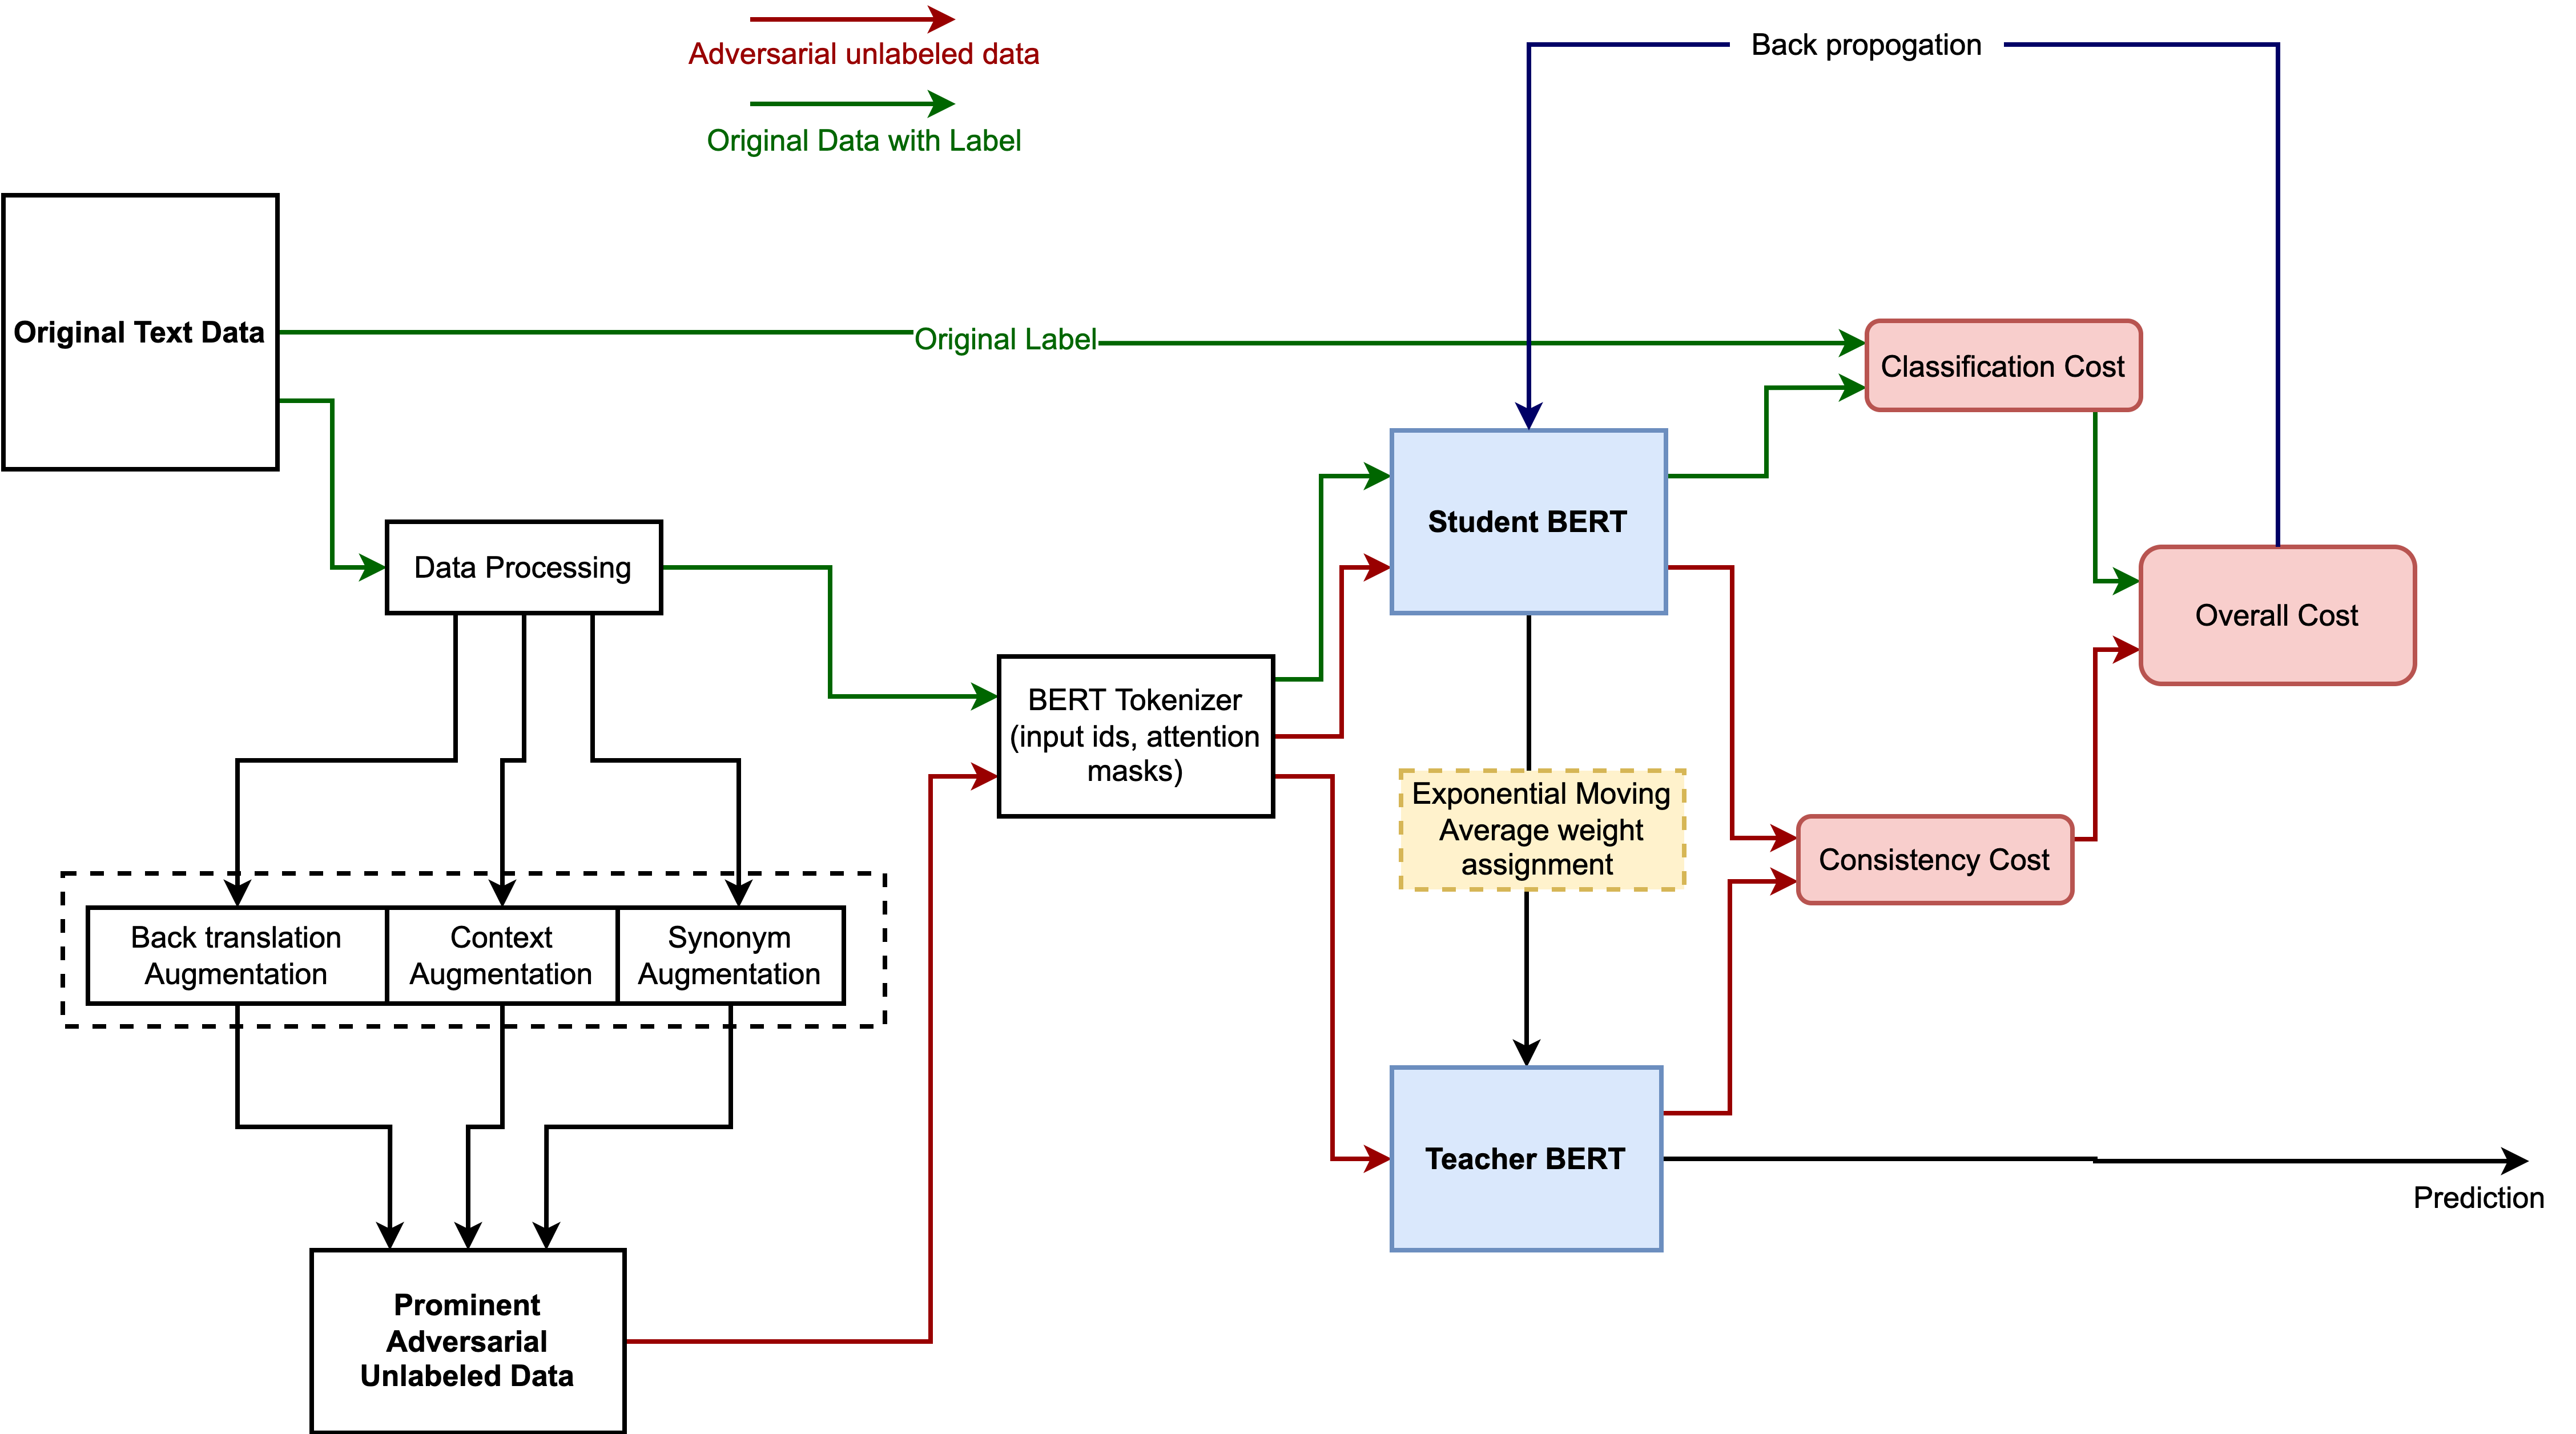
\includegraphics[width=1.1\textwidth]{img/Methodology.png}
     \caption{Proposed methodology }
     \label{diag:advMTBERT}
 \end{figure}

Training data is utilized to create prominent unlabeled adversarial samples and  three different data augmentation techniques are utilized 1) Synonym based, 2) Context based and, 3) Back translation based and discussed in length \ref{section:dataaugmentation}.  The label of those adversarial dataset is discarded hence called prominent unlabeled adversarial data. \\
\begin{algorithm}[h!]
    \caption{Mean Teacher Algorithm} \label{alg:MeanTeacher}
    \begin{algorithmic}
        \STATE \textbf{Data}: train set $\mathcal{(X,Y)}$,  Prominent Adversarial Unlabeled set($\mathcal{Z}$)
        \STATE \textbf{Hyper parameters}: \emph{r}, \emph{$\alpha$},\emph{epochs}
        \STATE \textbf{Create Model}: \emph{student($\theta$)}, \emph{teacher($\hat\theta$)} 
        \STATE  Train \emph{teacher} for n epoch
        \FOR{epochs = $1$ to $N$}
        \WHILE{$steps$}
        \STATE  \emph{student}($x$) = $y$\
        \STATE Compute Classification cost ($C(\theta)$) =Binary Cross Entropy($y$,$y')$
        \STATE  \emph{student}($z$) = $y_s$
        \STATE  \emph{teacher}($z$) = $y_t$
        \STATE Compute Consistency cost $J(\theta)$=Mean Squared Error($y_s$,$y_{t}$)
        \STATE Compute Overall cost  $\textit{O}(\theta)= r C(\theta)+(1-r)J(\theta)$
        \STATE Compute \emph{gradients}, \textit{O}($\theta$) w.r.t  $\theta$ 
        \STATE Apply \emph{gradients} to $\theta$
        \STATE Update Exponential Moving average of $\theta$ to $\hat\theta$ i.e. $\hat\theta_t= \alpha\hat\theta_{t-1}+(1-\alpha)\theta_t$\
        \ENDWHILE
        \ENDFOR
    \end{algorithmic}
\end{algorithm}
Erik et. al. \cite{englesson_consistency_2021}study revealed that model trained on noisy data exhibits a lower consistency that trained on clean data and reduces further if we increase the ratio of noise. However, including loss function during training which tries to reduce this consistency loss and can create comparatively robust model, hence called consistency regularization. The gradient based methods \cite{miyato_adversarial_2017} and the proposed approach both exploit the principle of consistency regularization \cite{tarvainen_mean_2018}. However, in text domain the later approach has not been studied hence, the inspiration behind the study.
Moreover, the motivation behind using the approach is to study the model performance by using comparatively simpler adversarial example and observing the impact of model in utilizing the capabilities of language models such as context writing and back translation. It is hypothesized that robustness can be achieved by learning more representations and regularize model by not letting to learn the deep insight of the representation to avoid over fitting as well. Furthermore, exponential moving average (EMA) plays crucial role in increasing generalization and performance under attack. 

\section{Text Attack Recipes and Tool (2 pages)}
\label{section:attackrecipes}
To evaluate the proposed approach, four black box attack recipes has been selected which satisfy lexical, grammatical, and semantic constraints. To utilize all the attack recipes
to evaluate baseline BERT model and proposed Mean Teacher BERT, we have TextAttack python package\cite{morris_textattack_2020}. is  In this section, we will discuss about
their attacking principle, working and characteristics.

\subsection{TextFooler}
\label{subsection:textfooler}
Di jin et$.$ al$.$ proposed Textfooler \cite{jia_certified_2019}, a simple and effective adversarial attack generation strategy in black box settings which has characteristic
of preserving the semantics, and grammar which they called utility-preserving adversarial examples as shown in figure \ref{diag:TextFoolerExp}. For better understanding,
we briefly explain the three steps process of generating adversarial attacks below:

\begin{enumerate}
    \item  \textbf{Word Importance Ranking}: Given sentence of words, they create ranking of each word by calculating change before and after deleting the words called importance
    score. Followed by filtering out stop words using NLTK and spaCy libraries just to preserve the grammar of the sentence.
    %\item \textbf{Word Transformer}: To replace the word with synonym, they have utilized novel word embeddings proposed by  Mrks�?ic �? et$.$ al$.$ \cite{mrksic_counter-fitting_2016}
    which is basically injects antonymy and synonymy into vector space representations to improve vectors capability of semantic similarity. The replacement policy completely depends
    on three constraint (1) Similar semantic similarity, (2) Fit within the surrounding context , (3) attacks the model. To calculate the similarity,  using Universal Sentence Encoder proposed
    by Cer et al. \cite{cer_universal_2018}, for encoding the sentence into high dimensional vector and calculating the cosine similarity between sentences. Then, selecting replacement
    candidates which has value above preset threshold value and create a pool of candidate.
    \item \textbf{Replacement}: Among pool of candidates, if there already exist any candidate that can alter the prediction of target model then candidate with highest cosine similarity
    score between original and adversarial sentence is selecting. Otherwise, lower confidence score of label  is selected.
\end{enumerate}

TextFooler, has accessed the performance of BERT model under adversarial attack  using IMDB movie review dataset . As per their experiment, the accuracy significantly dropped
from 90.9\% to 13.6 \% with perturbed words 6.1 , number of queries sent to target model 1134 and average length of the IMDB dataset 215. Furthermore,  TextFooler is computationally
inexpensive and complexity increases linearly with respect to text length.
\textit{TextFooler, a strong black-box attack baseline for text classification models. However, the adversarial examples generated by TextFooler solely account for the token level similarity via word embedding, and not the overall sentence semantics. This can lead to out-of-context and unnaturally complex replacements (see Table 3), which are }

\begin{figure}[h!]
    \centering
    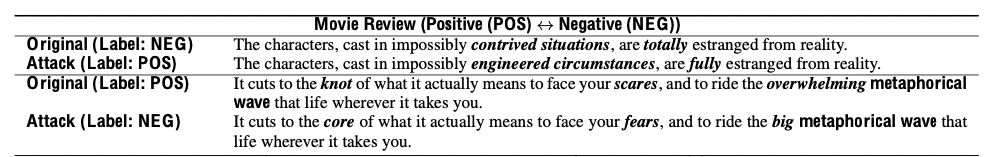
\includegraphics[width=.9\textwidth]{img/textfooler_example.png}
    \caption{TextFooler example  \cite{jia_certified_2019} }
    \label{diag:TextFoolerExp}
\end{figure}


\subsection{TextBugger}
\label{subsection:textbugger}
TextBugger  proposed by Jinfeng Li et$.$ al$.$ \cite{li_textbugger_2019}, is based on misspelling of words or characters which are visually and semantically similar to the original text
for human being. A simple misspelling can lead token to 'Unknown'  which is mapped to unknown tokens id can also force machine learning model to behave incorrectly. On the other
hand, studies shows that similar misspelling can still be perceptibly or inferred by the reader \cite{rawlinson_significance_2007,alzantot_generating_2018}  . This attack is focused on
both character-level and word-level perturbation. Jinfeng Li et. al has proposed both white box and black box attack generation strategies, however, our report is focused on black box
attack. Black box attack generation strategies is briefly discussed in Three steps:

\begin{enumerate}
    \item \textbf{Finding Important Sentences}: The importance score of individual sentences in an article is determined by confidence score of particular sentence by target model.
    \item \textbf{Finding Important Words}: The importance score of word is the difference between confidence of target model with word and without word.
    \item \textbf{Bugs Generation}: In TextBugger, they use five bugs generation strategy (1) \textbf{Insert}: Inserting space into words, (2) \textbf{Delete}: Deleting random character,
    (3) \textbf{Swap}: Swapping random adjacent character, (4) \textbf{Substitute-C}: Substitute character with visually similar characters, and (5)\textbf{ Substitute-W} : Replacing word with top-k nearest neighbour in context aware word vector space , as shown in figure \ref{diag:textbug}
\end{enumerate}

\begin{figure}[h!]
    \centering
    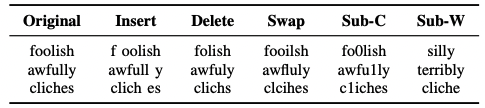
\includegraphics[width=.8\textwidth]{img/textbugger_5strat.png}
    \caption{TextBugger 5 bug generation strategies \cite{li_textbugger_2019} }
    \label{diag:textbug}
\end{figure}
TextBugger model is evaluated against LR, CNN, and LSTM  using IMDB movie review dataset, and have shown 95.2\%, 90.5\% and 86.7\% respectively, with perturbed word
4.9\%, 4.2\% and 6.9 \% respectively. However, observing the effectiveness against BERT model is still not evaluated and is explored in this report.
Unlike TextFooler, TextBugger computational complexity is sub-linear to text length and can generate adversarial attacks in comparatively less time.

\subsection{Generating Natural Language Adversarial Examples through Probability Weighted Word Saliency (PWWS)}
\label{subsection:generatingadversarialexample}
Shuhuai et al$.$\cite{ren_generating_2019} proposed method of synonym and named entity (NE) replacement method which is determined by the words saliency  and the
classification probability, and proposed a greedy algorithm called probability weighted word saliency(PWWS). To replace the word with the synonym is decided by significant
change in classification probability and at the same time have minimum word saliency. Their approach is mainly can be explained in two steps as follows:

\begin{enumerate}
    \item \textbf{Word Selection Strategy}:  Word saliency defined as degree of change in classification probability of the model if the word is set to
    unknown \cite{li_understanding_2017}. Calculating word saliency vector of each word in a text, and prioritizing the words according to degree of change in classification probability
    after replacement as well as minimum word saliency of that words.
    \item \textbf{Replacement Strategy}: To find the substitution, they used WordNet to find the synonym of the words.  And, if word is Named Entity(NE), then  replacing the
    NE with similar type NE appeared in opposite class.
\end{enumerate}
Finally, greedily iterate through words replacement to make model change the label. This approach has been evaluated with Word based CNN \cite{kim_convolutional_2014},
Bi-directional LSTM model, LSTM and Char-based CNN\cite{zhang_character-level_2016}, however, still have open scope for evaluating against language models. Considering
Bi-LSTM result , the accuracy dropped from 84.86 \% to 2.00\%   with perturbation 3.38\% for IMDB dataset, example is shown in figure \ref{diag:pwwsexp}. However, the
computational and time complexity of the proposed approach is comparatively higher than other discussed strategies.
\begin{figure}[h!]
    \centering
    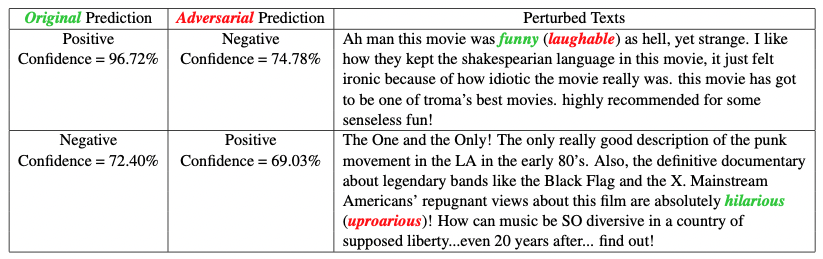
\includegraphics[width=.9\textwidth]{img/PWWSexample.png}
    \caption{Example attack of PWWS\cite{ren_generating_2019} }
    \label{diag:pwwsexp}
\end{figure}

\subsection{BAE: BERT-Based Adversarial Examples}
\label{subsection:bae}
Garg et al$.$\cite{garg_bae_2020} proposed a novel black box approach to generating adversarial examples by utilizing BERT masked language model(MLM). According to
their proposed approach, first they calculate words importance by computing the decrease in probability of predicting the correct label after deleting that particular word, similar
to Textfooler \cite{jia_certified_2019} and PWWS \cite{ren_generating_2019}. And, using pre-trained BERT MLM model, where a particular word is replaced with MASK
token and let the MLM model predict the context specific words. Then, filter  top K tokens based on most similarity score(Threshold 0.8) using Universal Sentence Encoder
\cite{cer_universal_2018} and removing words that doesn't fall into similar part-of-speech(POS) as the original word. Now, replacing the original word with top K(50) tokens,
iterate from most similar token in decreasing order until attack is successful and trying all combination. A schematic working diagram is shown in the figure \ref{diag:baeexp}.

\begin{figure}[h!]
    \centering
    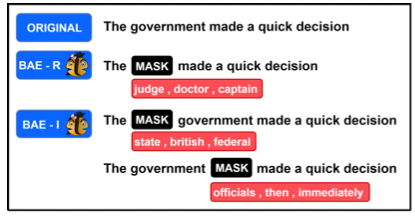
\includegraphics[width=.7\textwidth]{img/BAEexample.png}
    \caption{Schematic working and example of BAE\cite{garg_bae_2020} }
    \label{diag:baeexp}
\end{figure}

\section{Research Questions}
The main motivation behind the proposed methodology is to reveal using various data augmentation technique can enhance the performance of  language model under attack  without compromising on generalization. In other word, semi-supervised fine tuning of language models can create comparatively robust language models and language models still have scope of improvements. Precisely, the master thesis is trying to answer by creating teacher model using proposed semi-supervised approach and comparatively study the performance of conventional and proposed way of fine tuning in terms of generalization and under attack accuracy. The reason behind this hypothesis lies mainly in two concept, 1) averaging models weights over training steps tends to produce a more accurate model than using the final weights directly \cite{polyak_acceleration_1992} and teacher model is an average of consecutive student models thus teacher model should perform better. 2) The inclusion of data augmentation can enhance the robustness of the model \cite{belinkov_synthetic_2018} , hence the proposed approach should perform well in under attack too. \\
The robustness in this experiment would be measured using metrics like original accuracy, accuracy under attack, average word perturbation , average number of queries, and attack success rate which is discussed in length in \ref{section:metrics}. Hence, the hypothesis would be the proposed approach comparatively should have higher original accuracy, accuracy under attack and require higher number of queries and perturbation requirement to get attacked as well. And, comparatively lower attack success rate. Four different attack recipes are used to evaluate the model performance which is discussed in \ref{section:attackrecipes}. 
Furthermore, the experiment also tries to understand the robustness of model by studying the distribution of confidence score prediction under attack can reveal the resilience of  model towards attacks.  If model not allowing attack recipes to wrongly classify with higher confidence is a sign of robustness as well. 


%%%%%%%%%%%%%%%%%%%%%%%%%%%%%%%%%%%%%%%%%%%%%%%%%%%%%%%%%%%%%%%%%%%%%%%%%CHAPTER DATASET%%%%%%%%%%%%%%%%%%%%%%%%%%%%%%%%%%%%%%%%%%%%%%%%%%%%%%%%%%%%%%%%%%%%%%%%%
%%%%%%%%%%%%%%%%%%%%%%%%%%%%%%%%%%%%%%%%%%%%%%%%%%%%%%%%%%%%%%CHAPTER EXPERIMENTS%%%%%%%%%%%%%%%%%%%%%%%%%%%%%%%%%%%%%%%%%%%%%%%%%%%%%%%%%%%%%%%%%%%%%%%%%%%%%%%%%

\chapter{Experiment(7 pages)}
\label{chapter:experiment}

\section{Dataset (1-2 paragraph)}
\label{label:dataset}
For assessing the performance of baseline model and proposed model. We have selected two datasets, one is Covid-19 fake news  dataset provided at Codalab competition
and IMDB review binary classification dataset. IMDB dataset is sentiment classification dataset which contains movie reviews of the user and having two classes positive and
 negative and most generally used in classification and adversarial attack research papers. This dataset has 50,000 labelled but due to computational limitation, we have filtered
 and sampled only dataset whose length is in between 6 to 150 as augmentation process takes quite longer time which leads  6000 samples to train and evaluate our model. The
 train and test size is show in table \ref{table:train/test table }. And, we have sampled 6000 training labeled samples to create augmented unlabeled dataset.  Average length of the
 filtered dataset is 100.  The label distribution is completely balanced in training dataset.

Covid-19 Fake news dataset  is recent dataset specific for fake news detection tweets related to COVID 19 with label as fake and real.  Covid-19 fake news dataset size is 8000 and
we have completely utilized this dataset. Observing the performance of proposed model in more recent fake news dataset is motivation behind selecting the dataset. In contrast to
IMDB dataset, the average length of Covid-19 fake news dataset is 25 as mentioned in table \ref{table:Length stat }.

Covid-19 fake news dataset has mostly hashtags and less English words vocabulary which might create challenge for those recipes, we would like to investigate the performance
 of models under this scenario too. The label distribution is almost balanced as compared to IMDB dataset which is completely balanced. The intention is to observe the effect
 of label distribution.

\begin{table}[!h]
\centering
\begin{tabular}{ |c|c|c|c|c|c| }
\hline
Dataset & Train & Test & Unlabeled & Aug. Unlabeled \\
\hline
codalab (Positive/Negative) & 3199/2891 & 1071/969 & xxxx & xxxx \\
IMDB (Fake/Real) & xxxx/yyyy & xxxx/yyyy & xxxx & xxxx \\
\hline
\end{tabular}
\caption[Train/Augment test data]{Train/ Test split details of dataset }
\label{table:train/test table }
\end{table}

\section{Data Pre-processing and Exploration (3 pages)}
\label{section:datapreproc}
As language models are based on learning the context of the sentences hence least affected by stop words and removing those words might affect the performance. Hence,
the one of the benefit of language model is its negligible requirement of data cleaning or no data cleaning. In our case we have performed following data pre-processing steps:
\begin{enumerate}
\item  HTML tags removal.
\item Digit removal.
\item Lower casing.
\item  Punctuation removal.
\end{enumerate}

For achieving the particular task, we have utilized texthero python library which provide function related to data pre-processing and exploration.

\subsubsection{Data Exploration (3 pages)}
\label{subsection:dataexploration}
For training the mentioned models, we selected almost equal distribution of label in training data  and test data, and same training data we have utilized to create
unlabeled augmented data for training via proposed method as shown in \ref{table:train/test table }.

\begin{table}[!h]
\centering
\begin{tabular}{ |c|c| }
\hline
Dataset &  Avg. Length  \\
\hline
codalab & xxxx  \\
IMDB & xxxx  \\
\hline
\end{tabular}
\caption[Train/Augment test data]{Train/ Test split details of dataset }
\label{table:Length stat }
\end{table}

\section{Data Augmentation}
\label{section:dataaugmentation}
For creating the unlabeled augmented dataset, we have utilized three strategies :
\begin{enumerate}
\item  Synonym Augmentation
\item Context Based Augmentation
\item Back translation.
\end{enumerate}
The reason behind calling this dataset unlabeled augmented dataset is while augmenting the dataset there are high chance that the information is changed or completely opposite in contrast to label. Therefore, once we augment the data , we will not be using the label of augmented data hence unlabeled augmented dataset. During experiments, various python packages like text attack , nlpaug, and various basic python packages for synonym changes were tried. But, in the end , considering the time and computation constraint,  we have selected nlpaug data augmentation package to achieve all three augmentation strategies and can be accessed in following link. To augment the dataset, we have taken train dataset with dropping the label columns , then we randomly split this dataset into three part. One part for synonym augmentation, second part for context based augmentation, and remaining for back translation. \\ 
There was one more idea to create unlabeled data using different attack recipes, which might can give better result under attack. But, the motivation behind not using attack recipes because of assumption  that model is created with no or little understanding of nature of attacks. If we have implemented a particular attack recipe to create unlabeled data then, it might increase the robustness for specific attack recipes but overall evaluation of model performance would be biased and we want it completely random.\\
For synonym augmentation, wordNet lexical English database is used as augmentation source which consist of word definitions, hyponyms, and semantic relationship. Same database in our case utilized for synonym replacement. Parameter maximum augmentation($aug\_max$) is used to control the level of augmentation. It is set to 50 and 15 for IMDB  and Covid-19 fake news dataset respectively. One more parameter called \textit{iter} is utilized to create two different copies of synonym augmentation dataset.\\
TODO: Image of synonym augmentation. \\
Context based augmentation is based on replacing the words the words in the sentence without changing the  context. Generally, language models are used to achieve this particular task, hence it is quite time and memory expensive. Therefore, DistilBert language model is utilized to perform this augmentation. \\
Back translation is the process of converting sentences in different languages and then translating back to original language.  Like, context based augmentation, Marian translation framework is utilized , hence time and memory expensive. In our experiment, we are converting sentence into Romance language and back to English. We have used CITE model to perform this experiments. Marian translation framework is comparatively an free, faster and efficient . \\
TODO: Image for Back translation.
\section{Experiment Environment description (1-2 paragraph)}
To successfully perform experiments, Google colab notebook with GPU is utilized to perform the experiments.
TODO: GPU details need to mention or image.

\subsection{ Hyper parameter Details (1 paragraph)}
\label{subsection:hyperparameter}
 As shown in table \ref{table:HyperparameterTable}, to train the baseline model and proposed model, we have used these parameter values. However, observing the performance with different settings is not the current focus  and open for future task.
\begin{table}[!h]
\centering
\begin{tabular}{ l c c }
\hline
Hyper parameter 		& \multicolumn{2}{c}{Used parameters in this work}\\
\hline
Optimizer 				& \multicolumn{2}{c}{Adam} \\
Learning rate 			& \multicolumn{2}{c}{ $2\epsilon -5$ } \\
Loss function 			& \multicolumn{2}{c}{Binary Cross Entropy}  \\
Epochs 				& \multicolumn{2}{c}{$3$} \\
Batch Size 			& \multicolumn{2}{c}{4 } \\
Loss Ratio 			&\multicolumn{2}{c}{0.5}\\
Alpha 			&\multicolumn{2}{c}{0.99}\\
Dropout  			& \multicolumn{2}{c}{0.2}  \\
Max length 			 & \multicolumn{2}{c}{100}  \\
\hline
\end{tabular}
\caption[Hyper-parameters with test run results]{Hyper-parameters Details}
\label{table:HyperparameterTable}
\end{table}


\section{Metrics }
\label{section:metrics}

In the experiment, the generalization of the model is calculated using  accuracy of the target model on original test samples, here it would be referred as original accuracy. Original accuracy is percentage of correct prediction over complete test samples. \\
Then, robustness of the target models is calculated using 4 different metrics 1) Accuracy under attack, 2) Average word perturbation 3) Average number of queries and 4) Perturbation Score. Accuracy under attack is the percentage of correct prediction over test samples i.e  accuracy of the target model against crafted test samples.  Comparison of original accuracy and accuracy under attack can provide significant information about efficiency of the target model and attack recipes as well. If more significant difference between both metrics signals the lower robustness against attack. The attack success rate is also counter part of accuracy under attack which reveals the success of attack recipes. \\
Another metric apart from accuracy, the average perturbed word in percentage is noted which is average number of words need to change in order to get successful attack. Generally, higher word perturbation signals lower robustness and this metric also depends on text length. \\
Additonally, average number of queries is the average of number of times attacks recipes send perturbed text samples to the target models for successful attack. More the average number of queries leads higher robustness against attack. \\
Moving forward, perturbation score which is confidence score or predicted probability of the target models under attack. According to hypothesis, the only for successful attacks, lower the mean  signals higher robustness . \\

\section{Threat Model}
\label{section:threadmodel}

In this experiment, the attack recipes are selected based of level of knowledge, target, level of perturbation, and assumptions. 
As most of the attack are basically done under black box setting, the attacks recipes are only exposed to the target model output and test samples from same corpus.  Under this black box setting, the attacker can only query the target model with perturbed inputs and getting the corresponding confidence score or predictions . And, the attacker is not aware of the model architecture, parameters, or training data. It can only query the target model with supplied inputs. As test samples is from original corpus of the data, hence that the present test samples has extracted from different corpus is an assumed.
It is also assumed that attacker has the access to similar baseline model. As the tokenizer used while training i.e. from huggingface \cite{noauthor_hugging_nodate}  open source python package for language models, similar tokenizer  is initialised from same package.\\
Evaluation of the model is only performed in binary classification task, hence the attacks are mainly un-targeted but, because of binary classification it is assumed as targeted classification.  And, only word level and multi-level which includes word and char level of word perturbation are considered. As, most of attacks are basically word level and character level hence, clear the intent of this selection.\\
The robustness of target models is evaluated using four attack recipes mentioned in\ref{section:attackrecipes}, hence it is assumed that attacker has access to  those attack recipes and the performance of  model could be different if some other attack recipes are utilized.  Furthermore, it is also assumed that the attack test samples are syntactically and semantically similar as per the claimed based on the attack recipes paper , hence, similarity metrics are not included in the experiment.
The model is trained of mentioned settings \ref{subsection:hyperparameter}, and model can perform better or worse in different settings.
Moving forward, about the transferability of the proposed approach , as the experiment is performed on two different language models differ in pre-training, it is assumed that the approach would also perform the same if some other language models are utilized. 
%%%%%%%%%%%%%%%%%%%%%%%%%%%%%%%%%%%%%%%%%%%%%%%%%%%%%%%%%%%%%%%%CHAPTER RESULT ANALYSIS%%%%%%%%%%%%%%%%%%%%%%%%%%%%%%%%%%%%%%%%%%%%%%%%%%%%%%%%%%%%%%%%%%%%%%%%%%
\chapter{Result Analysis (3 pages)}
\label{chapter:result}
According to experiment result of both the datasets shown in table  \ref{table:IMDBExpRes} and \ref{table:FakeNewsExpRes}, the proposed approach i.e. MTBERT  has outperformed all the other language models considering all the metrics. If comparing proposed versus baseline model, the MTBERT and MTDistilBERT model has also performed better than respective baseline models i.e. BERT and DistilBERT.  
MT BERT model has shown 1-2\% improvement  in original accuracy than baseline model in both the datasets as shown figure \ref{fig:moaandauaimdb}. Proposed model has shown  25-30\% improvement in accuracy under attack at the same instance require considerably higher number of queries and word perturbation and in other words, has shown lowest drop in original accuracy. In opposite, BERT and DistilBERT has shown lowest performance considerably require less number of queries and overall word perturbation. 
\begin{figure}[h!]
    \centering
    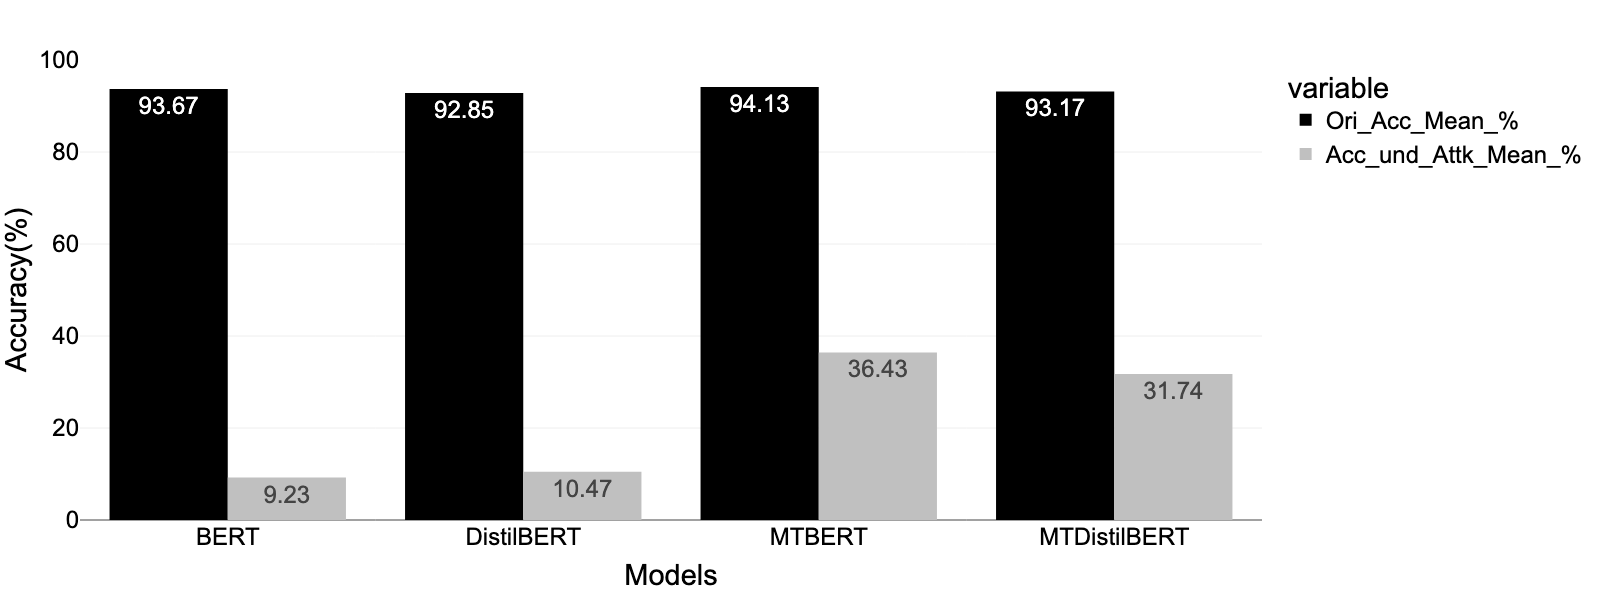
\includegraphics[width=0.7\linewidth]{img/MOAandAUA_Imdb}
    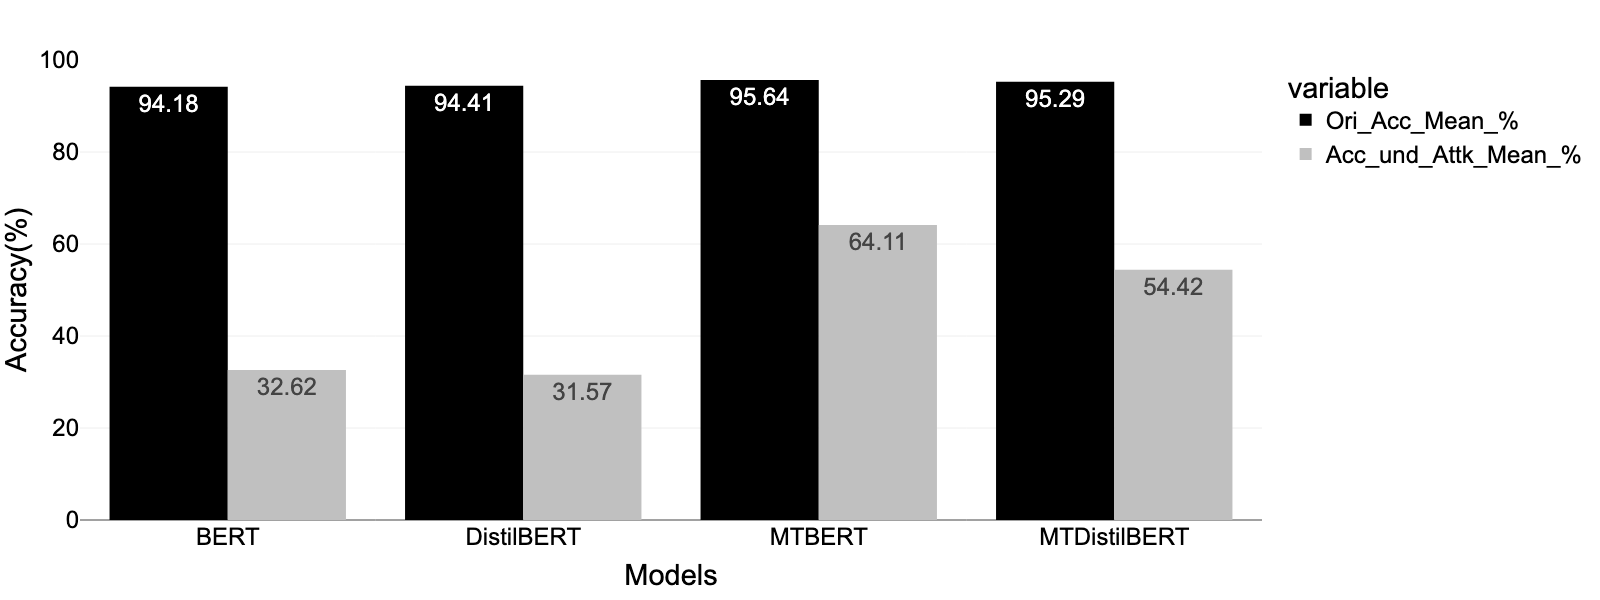
\includegraphics[width=0.7\linewidth]{img/MOAandAUA_fknews}
    \caption{Original accuracy and Accuracy under attack comparison plot.}{MTBERT has shown better performance in both metrics followed by MT DistilBERT. Baseline models (BERT and DistilBERT) has shown highest drop in accuracy when under attack , however, proposed models have shown significant robustness against attack. }
    \label{fig:moaandauaimdb}
\end{figure}

\begin{table}[h!]
    \centering
    \hspace*{-1.2em}
    \resizebox{1.0\textwidth}{!}{
        \begin{tabular}{|c|c|c|c|c|c|c|}%{|l|l|r|r|r|r|r|}
            \toprule
            Attack Recipe&Model&  Acc. und Attack(\%) &  Acc. Succ. Rate(\%) &   Avg. Pert. Word(\%) &   Avg. No. Queries &  Ori. Acc.(\%) \\
            % Attack Recipe & Model &                     &                     &                      &                    &               \\
            \toprule
            BAE & BERT &		 33.93 &               63.77 &                 3.78 &             242.24 &         93.67 \\
            & DistilBERT &               33.25 &               64.18 &                 3.56 &             238.20 &         92.80 \\
            & MT BERT &               56.45 &               40.03 &                 3.55 &             198.26 &         94.13 \\
            & MT DistilBERT &               53.50 &               42.51 &                 3.31 &             285.70 &         93.05 \\
            \midrule
            PWWS & BERT &                0.60 &               99.36 &                 3.97 &             749.33 &         93.67 \\
            & DistilBERT &                1.70 &               98.17 &                 3.98 &             750.12 &         92.80 \\
            & MT BERT &               23.20 &               75.35 &                 5.70 &             890.84 &         94.13 \\
            & MT DistilBERT &               17.55 &               81.14 &                 5.37 &             867.65 &         93.05 \\
            \midrule
            TextBugger & BERT &                2.30 &               97.54 &                22.04 &             235.27 &         93.67 \\
            & DistilBERT &                5.45 &               94.03 &                20.80 &             258.47 &         92.80 \\
            & MT BERT &               35.13 &               62.68 &                28.57 &             449.96 &         94.13 \\
            & MT DistilBERT &               30.05 &               67.70 &                26.66 &             420.39 &         93.05 \\
            \midrule
            TextFooler & BERT &                0.10 &               99.89 &                 5.14 &             279.12 &         93.67 \\
            & DistilBERT &                1.07 &               98.85 &                 5.07 &             278.73 &         92.85 \\
            & MT BERT &               30.92 &               67.16 &                 8.04 &             720.77 &         94.13 \\
            & MT DistilBERT &               25.48 &               72.64 &                 7.54 &             613.91 &         93.17 \\
            
            \bottomrule
        \end{tabular}
    }
    \caption[Experiment Result]{IMDB datasets experiment result. MTBERT model has performed well overall and shown comparatively better robustness towards attack. }
    \label{table:IMDBExpRes}
\end{table}

\begin{table}[h!]
    \hspace*{-1.2em}
    \resizebox{1.0\textwidth}{!}{
        \begin{tabular}{|llrrrrr|}
            \toprule
            Attack Recipe& Model&  Acc. und Attack(\%) &  Acc. Succ. Rate(\%) &   Avg. Pert. Word(\%) &   Avg. No. Queries &  Ori. Acc.(\%) \\
            %Attack Recipe & Model &                     &                     &                      &                    &               \\
            \toprule
            BAE & BERT &               67.40 &               28.30 &                20.43 &              82.32 &         94.00 \\
            & DistilBERT &               67.53 &               28.46 &                18.86 &              79.08 &         94.40 \\
            & MT BERT &               77.60 &               18.83 &                16.54 &              88.56 &         95.60 \\
            & MT DistilBERT &               74.00 &               22.24 &                19.46 &              86.40 &         95.17 \\
            \midrule
            PWWS & BERT &               24.50 &               73.94 &                20.23 &             214.95 &         94.00 \\
            & DistilBERT &               25.40 &               73.09 &                19.28 &             210.40 &         94.40 \\
            & MT BERT &               59.47 &               37.80 &                17.90 &             236.99 &         95.60 \\
            & MT DistilBERT &               48.87 &               48.65 &                18.70 &             227.90 &         95.17 \\
            \midrule
            TextBugger & BERT &               31.27 &               65.74 &                24.77 &              82.49 &         94.00 \\
            & DistilBERT &               25.57 &               72.92 &                22.54 &              76.61 &         94.40 \\
            & MT BERT &               65.87 &               31.10 &                23.45 &             114.34 &         95.60 \\
            & MT DistilBERT &               54.23 &               43.01 &                24.57 &              96.05 &         95.17 \\
            \midrule
            TextFooler & BERT &                7.53 &               91.98 &                22.52 &             180.88 &         94.00 \\
            & DistilBERT &                7.47 &               92.09 &                21.40 &             164.27 &         94.40 \\
            & MT BERT &               54.13 &               43.38 &                21.24 &             283.06 &         95.60 \\
            & MT DistilBERT &               42.27 &               55.57 &                24.45 &             198.96 &         95.17 \\
            \bottomrule
        \end{tabular}
    }
    \caption[Experiment Result]{  Fake news dataset: MTBERT model has performed well overall and shown comparatively better robustness towards attack.  }
    \label{table:FakeNewsExpRes}
\end{table}
Now, if we discuss about the performance of model considering individual metrics metrics. MTBERT  require comparatively higher number of queries to get attacked. As shown in figure \ref{fig:avgnquebyattackrecipes}. BAE attacks has shown lowest requirements for queries followed by TextBugger, but also found out to be least effective in attacking. Overall, PWWS need significantly higher number of queries followed by TextFooler and also found out to be effective in attacks. Furthermore, both attack recipes has shown positive dependencies on text length,if we observer the considerable difference in queries for both the datasets \ref{fig:avgnquebyattackrecipes}. However, BAE and TextBugger shown least difference with respect to text length. 
In another point, considering only TextFooler attack recipe, the difference between proposed and baseline models queries also increases with respect text length. In fake news dataset, TextFooler number of queries difference between BERT and MTBERT is less but doubled in IMDB datasets. As shown in table \ref{table:numqueries}, the proposed model has mean value VALUE and VALUE compared to V1 and V2 a difference of and have broader distribution than baseline model.  It is evident that model created by proposed approach required higher number of queries, and the difference is clearly visible in IMDB datasets. 
\begin{figure}[h!]
	\centering
	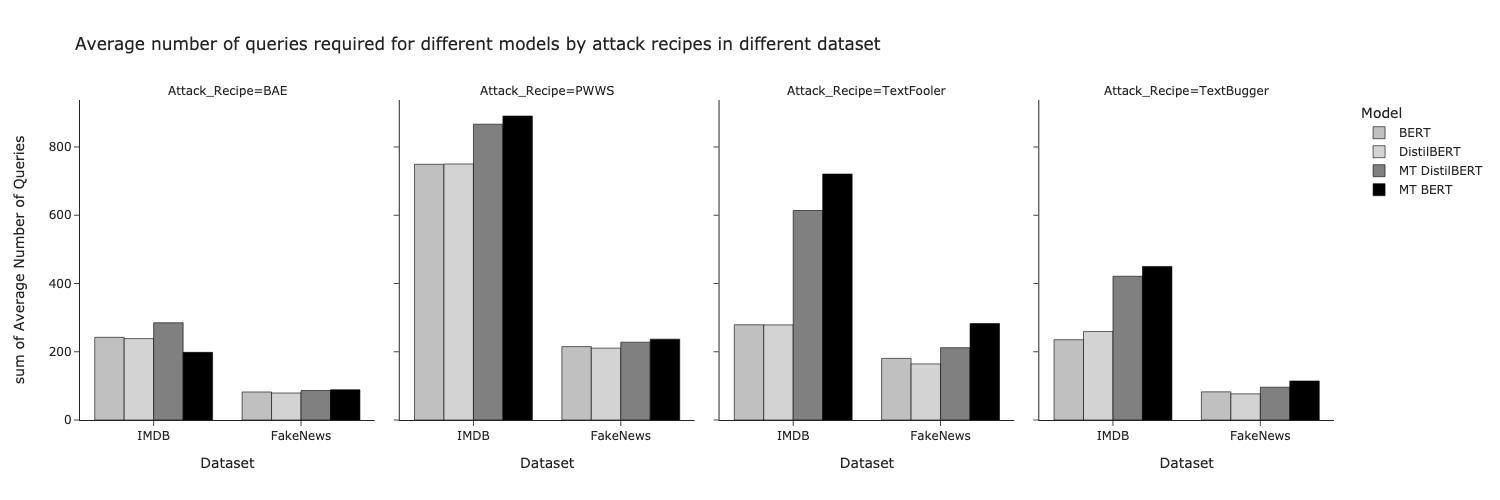
\includegraphics[width=1.0\linewidth]{img/AvgNQuebyAttackRecipes}
    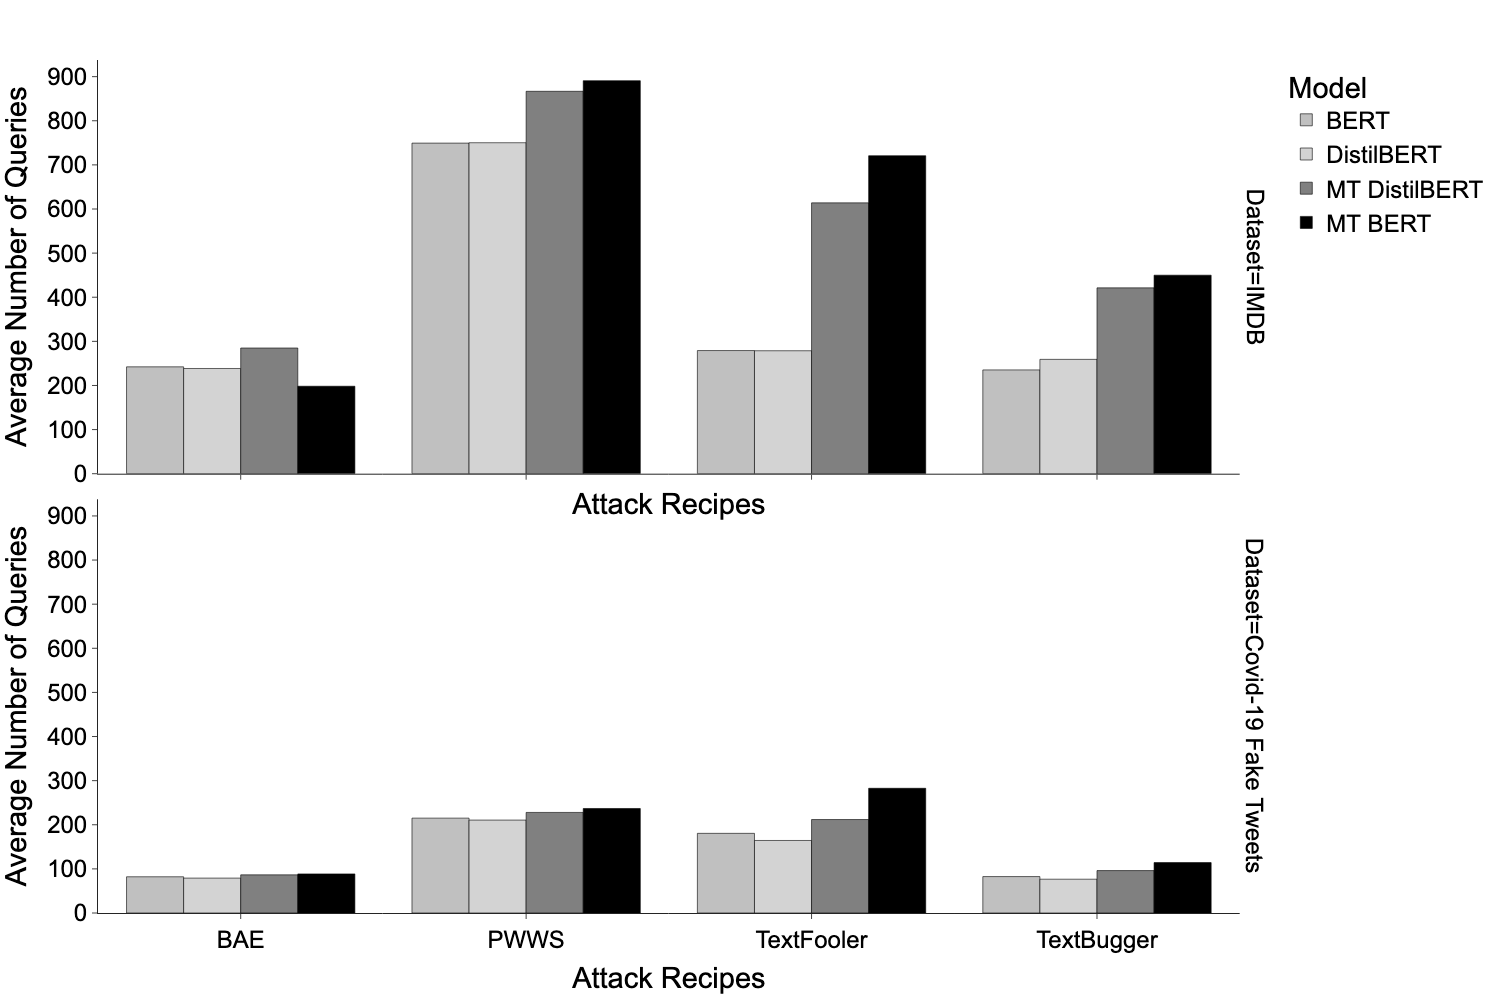
\includegraphics[width=1.0\linewidth]{img/AvgNQuebyDataset}
	\caption{Number of queries with respect to datasets and attack recipes.}{ PWWS has shown highest overall number of queries requirement followed by TextFooler.  And, we can observe how number of queries increases with respect to text length.}
	\label{fig:avgnquebyattackrecipes}
\end{figure}

\begin{table}[h!]
    \centering
    \hspace*{-0.7em}
    \resizebox{1.0\textwidth}{!}{
        \begin{tabular}{lllrrrrrrrr}
            \toprule
            {} &   Dataset &         model &     count &   mean &    std &   min &    25\% &    50\% &    75\% &      max \\
            \midrule
            0 &   &          BERT &  7,005.00 & 160.17 & 114.93 & 10.00 &  75.00 & 130.00 & 214.00 &   885.00 \\
            1 &  FakeNews &    DistilBERT & 12,096.00 & 138.74 & 100.89 & 10.00 &  63.00 & 110.00 & 188.00 &   945.00 \\
            2 &   &        MTBERT &  3,143.00 & 138.50 & 115.72 & 13.00 &  58.00 &  99.00 & 181.00 &   708.00 \\
            3 &   &  MTDistilBERT &  7,373.00 & 142.82 & 122.53 & 10.00 &  56.00 & 103.00 & 188.00 & 1,075.00 \\
            \midrule
            4 &       &          BERT & 16,101.00 & 361.27 & 282.52 & 24.00 & 161.00 & 232.00 & 507.00 & 1,841.00 \\
            5 &      IMDB &    DistilBERT & 16,608.00 & 410.52 & 309.74 & 24.00 & 164.00 & 264.00 & 667.00 & 1,708.00 \\
            6 &       &        MTBERT & 10,316.00 & 434.36 & 334.49 & 24.00 & 165.00 & 297.00 & 674.00 & 2,207.00 \\
            7 &       &  MTDistilBERT & 12,287.00 & 411.52 & 340.87 & 24.00 & 158.00 & 253.00 & 634.50 & 2,128.00 \\
            \bottomrule
        \end{tabular}
    }
    \caption[Number of queries score table ]{Queries descriptive statistics of successful attack. Proposed models require higher number of queries in contrast to baseline model.   }
    \label{table:numqueries}
\end{table}
%\begin{figure}[h!]
%    \centering
%    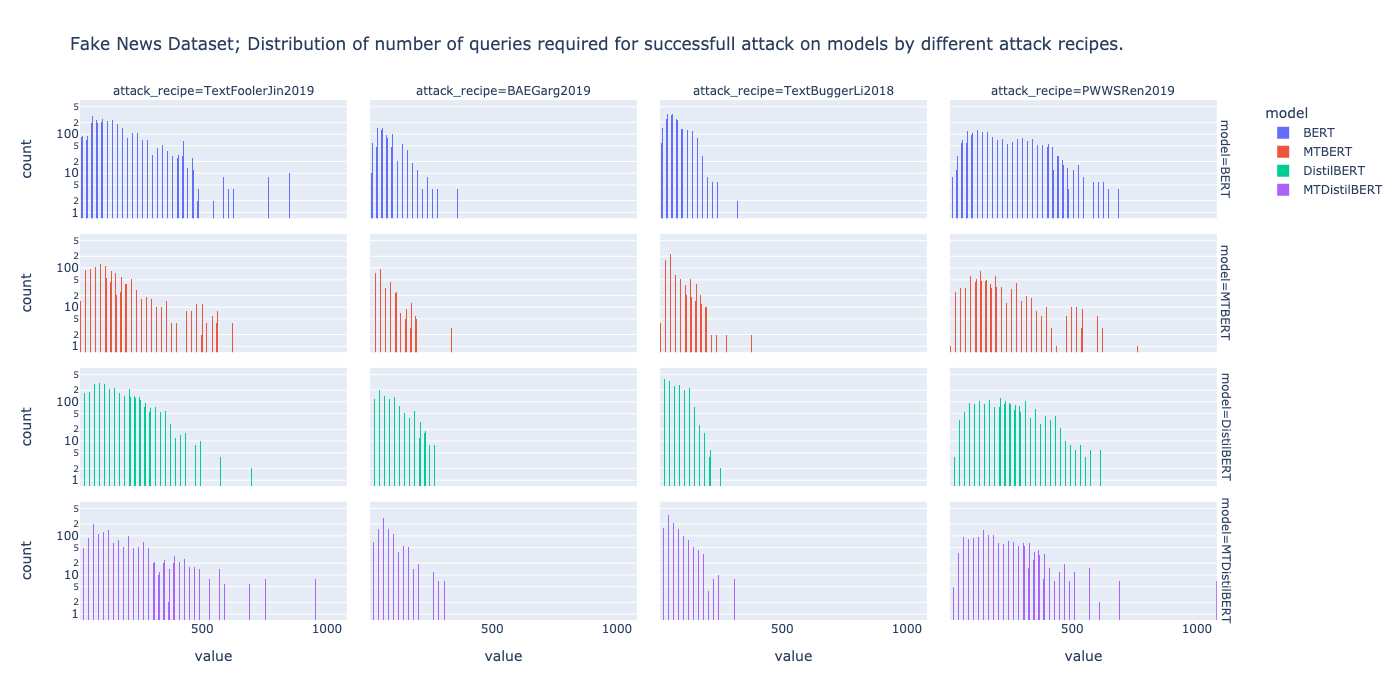
\includegraphics[width=1.1\linewidth]{img/NumQueriesDist_fknews}
%    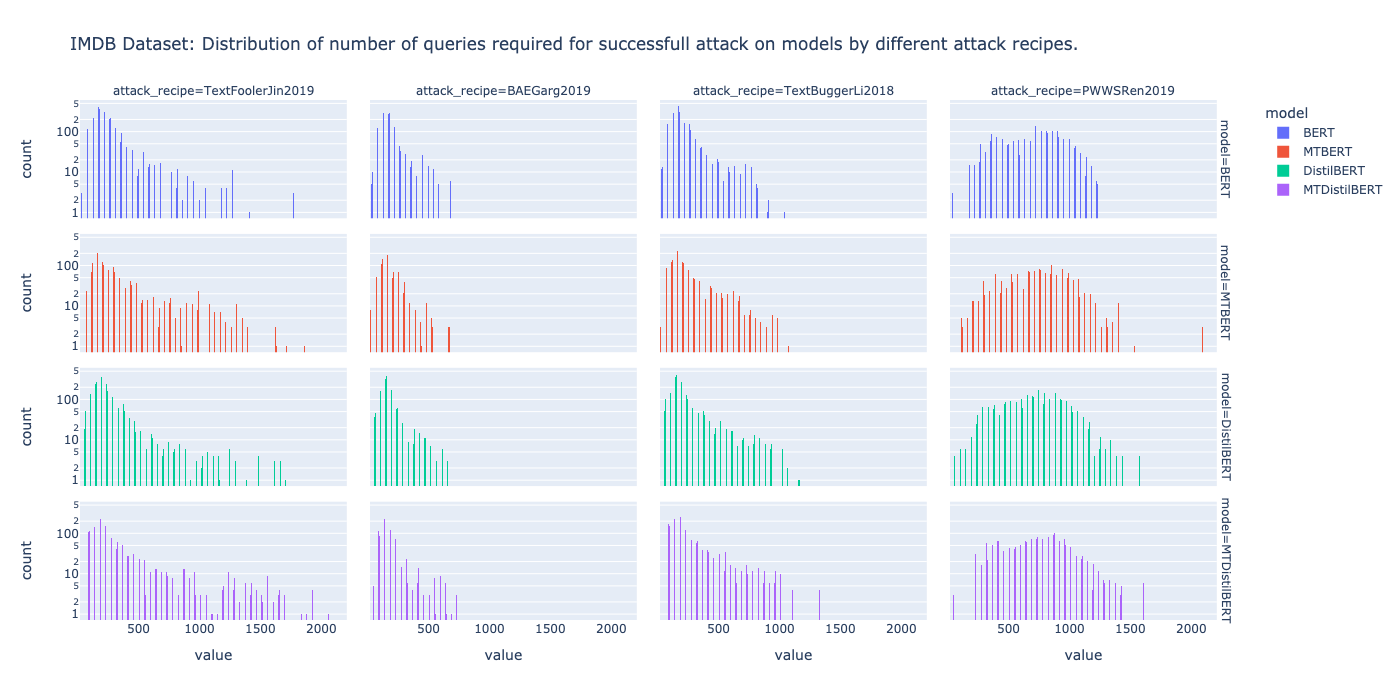
\includegraphics[width=1.1\linewidth]{img/NumQueriesDist_IMDB}
%    \caption{}
%    \label{fig:numqueriesdistfknews}
%\end{figure}


To understand the robustness of  models with respect to word perturbation, less significant difference is observed. In fake news dataset, the average word perturbation required by proposed models is comparatively higher , however, for IMDB dataset it is opposite.  The difference in word perturbation in both dataset is higher, and IMDB dataset has shown higher words perturbation in contrast of Fake news dataset  except TextBugger which has shown almost same perturbation rate.TextBugger require higher number of word perturbation followed by TextFooler. On the other hand, BAE required lowest number of perturbation followed by PWWS.
\begin{figure}[h!]
    \centering
    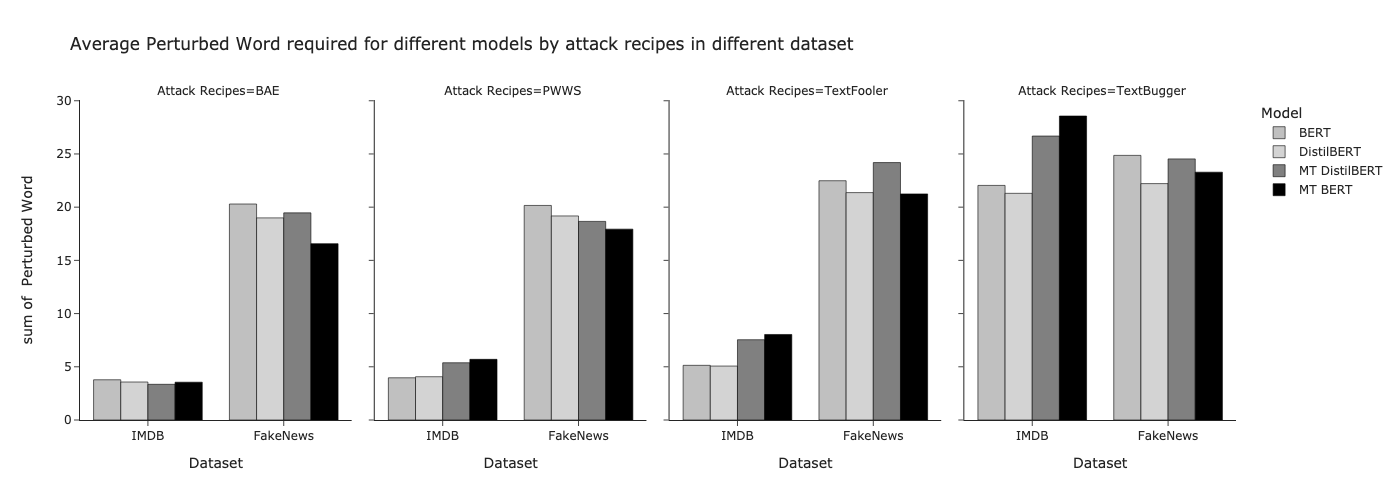
\includegraphics[width=1.0\linewidth]{img/AvgPertByAttackRecipes}
    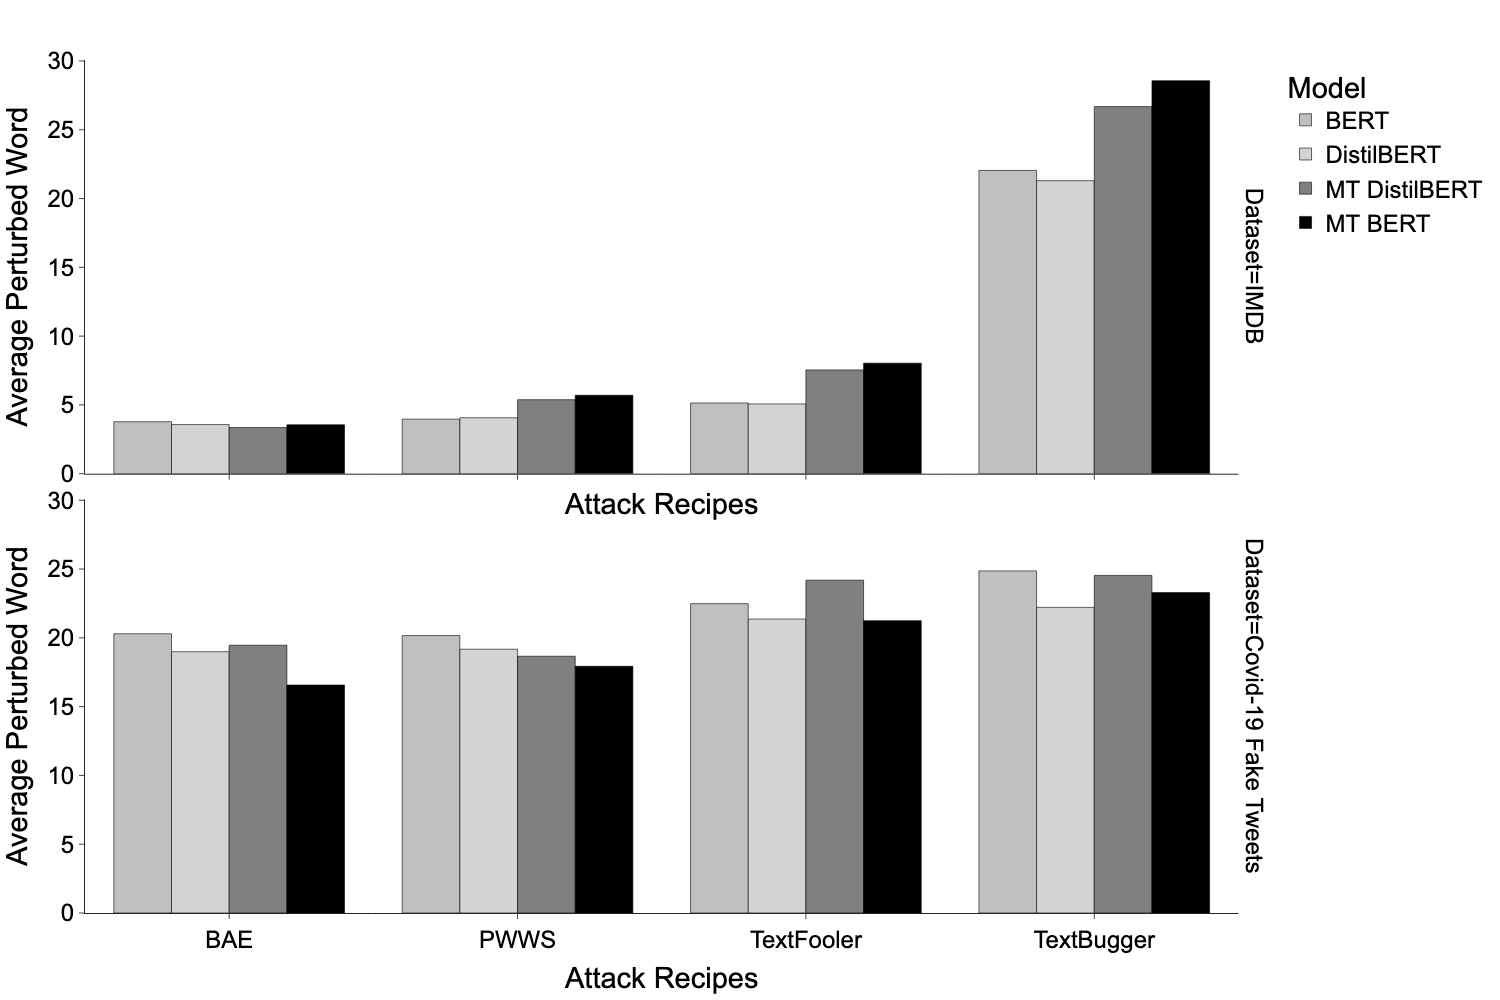
\includegraphics[width=1.0\linewidth]{img/AvgPertByDataset}
    \caption{Word perturbation as per datasets and attack recipes}{ TextBugger has shown highest word perturbation in both the datasets and also shown less difference between both dataset. However, BAE has lower word perturbation followed by PWWS attack recipe. Except TextBugger huge difference of word perturbation between datasets is observed. Fake news dataset has shown significantly higher word perturbation requirements.  }
    \label{fig:avgpertbyattackrecipes}
\end{figure}

Intuitively, while running the experiments we logged perturbation score that is predicted probability under attack in other term confidence score. To answer the question, how much proposed 
 and baseline model let the attacker to change the confidence score of successful attacks. As shown in figure \ref{fig:pertscoredist}, the distribution of proposed model is comparatively more left shifted than baseline models. The proposed model does not let attack recipe go beyond a particular limit i.e. 0.70 \ref{table:perturbationscore}, however, baseline models are more uniform and shown less resilience.  
 The mean and  range of MT BERT model is 0.53 and 0.50 to 0.55 , but for BERT model 0.59 and 0.50 to 0.66, which is a significant improvement in the model. 
\begin{figure}[h!]
    \centering
    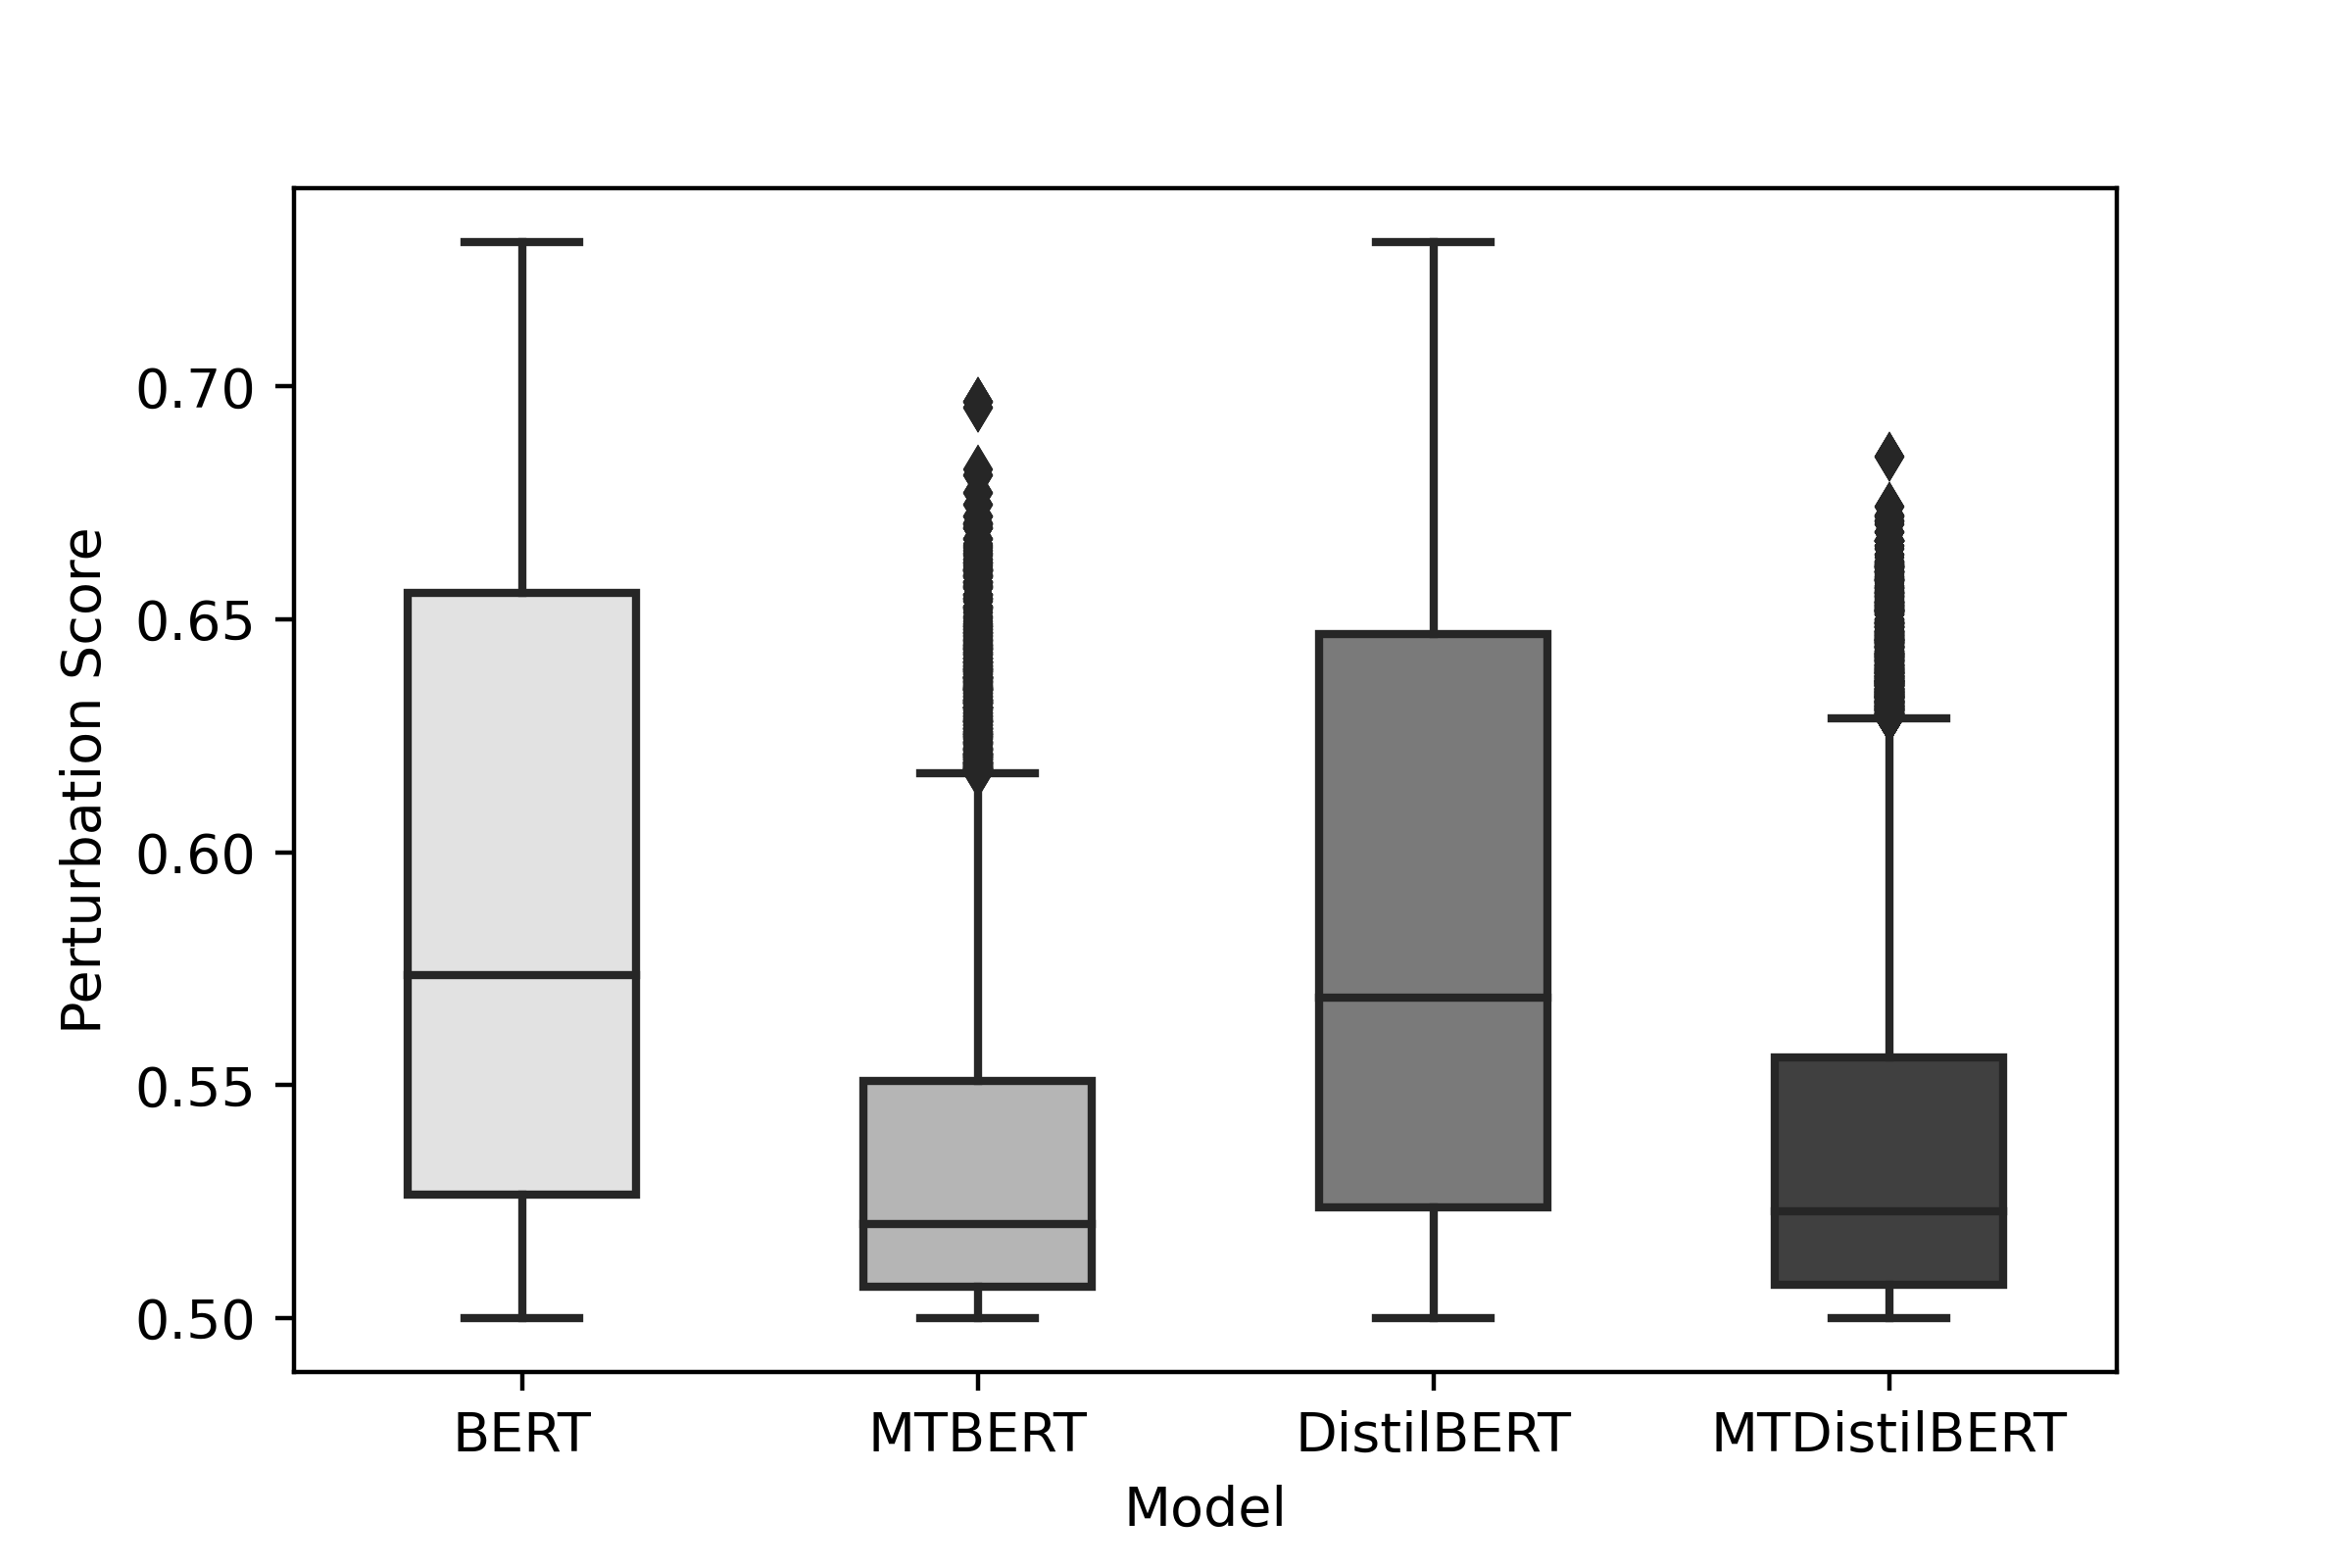
\includegraphics[width=1.0\linewidth]{img/PertScoreDist}
    \caption{Perturbation Score Distribution}{ The Proposed model are comparatively more left shifted and collected in range of 0.50 to 0.55 i.e 10 \% improvement compared to baseline model.}
    \label{fig:pertscoredist}
\end{figure}

\begin{table}[h!]
    \centering
    \hspace*{-0.7em}
    \resizebox{1.0\textwidth}{!}{
        \begin{tabular}{llrrrrrrrr}
            \toprule
            {} &         model &     count &  mean &  std &  min &  25\% &  50\% &  75\% &  max \\
            \midrule
            0 &          BERT & 38,507.00 &  0.59 & 0.07 & 0.50 & 0.53 & 0.57 & 0.66 & 0.73 \\
            1 &    DistilBERT & 47,222.00 &  0.59 & 0.07 & 0.50 & 0.52 & 0.57 & 0.64 & 0.73 \\
            2 &        MTBERT & 22,262.00 &  0.53 & 0.04 & 0.50 & 0.51 & 0.52 & 0.55 & 0.70 \\
            3 &  MTDistilBERT & 32,012.00 &  0.54 & 0.04 & 0.50 & 0.51 & 0.52 & 0.56 & 0.67 \\
            \bottomrule
        \end{tabular}
  }
    \caption{Perturbation score table }{Perturbation score descriptive statistics of  successful attacks combining both dataset. Proposed model has shown significant improvement over baseline model. 
        And, mostly in limited in range 0.53-0.70 and 75 \% of attacks score is under 0.55 a sign of robustness.}
    \label{table:perturbationscore}

\end{table}
In case of attack recipes, MT BERT has shown highest robustness towards all attack recipes. However, especially highest in BAE attack recipes and lowest in PWWS and TextFooler(still higher than other models.
PWWS and TextFooler are more successful in attacking the models considering both dataset. However, MT BERT has shown highest robustness compared to other mentioned models.
\section{Discussing on Research Questions}
As per the experiment result and analysis , the baseline model has outperformed considering all metrics and attack recipes, and shown significant robustness against attacks. The proposed approach comparatively has shown notable improvement in generalization and also significantly lower attack success rate. Additionally, require comparatively higher word perturbation rate , number of queries and perturbation score is also limited in lower range. Which answer to the question that 
the language model trained with noisy data and including loss function called consistency loss while training could result in better generalization and robustness than fine-tuned in conventional way as it is achieved by gradient based method. The mean teacher as proposed by \cite{tarvainen_mean_2018} in image- domain can show similar result in text-domain , if suitable noisy data specific to text is included.  In the end, opens the scope of improvements in language models either during pre-training or fine tuning. \\
Answering to the question of why proposed approach works, is because of including only noisy data in training samples would not actually lead to lower generalization, but at the same time if we include respective loss function which optimizes weights according to both classification and consistency loss can help model avoiding over-fitting and wont let model to learn deep insight of data. And, at the same time let model learn broad level of representation by including many noisy word synonym. Which also backs points made by on consistency regularization via noisy data  \cite{belinkov_synthetic_2018,englesson_consistency_2021}.  As the experiment performed in two different models, i.e. BERT and DistilBERT also proves its transferability to other language models. 


\chapter{Limitation, Future Work and Conclusion}
\label{chapter:conclusion}

\section{Limitations}
\label{section:limitations}
One of the major challenges in generating text samples are, unlike image domain the perturbation can be made impreceptible to human but in case of text domain achieving similar level of imperceptibility is still a open challenge due text data discrete nature. Most of the researches claimed to manage similar level of syntactic and semantic of the original text, but, in reality, those attack samples can be recognizable to human.\\
 The attacks, data augmentation technique, and semi-supervised training approaches implemented in image-domain can not be directly utilized in text domain, hence, it still require separate effort and contribution to implement it into the text-domain and observer their performance. 
In the experiment, the proposed approach has shown comparatively better performance than conventional model, but, does not claim to be robust to all types of attacks. Till now, no defense strategy can handle all different types of attacks as the nature of attack is not known. And, including respective noisy data can improvement robustness against  its corresponding attacks. \\
Till now in security domain in text-domain, no standard evaluation metrics and framework present to compare different researches and strategies which demand focused research on this particular domain. In another case,   the recent researches are more focused on increasing model generalization, than study the of those approaches in models robustness are not studied.


\section{Future Work }
\label{section:futurework}
The evaluation of the proposed approach could be performed to evaluate more recent state-of-art language models, and the work could also concentrate on hypothesis that extreme pre-training of language model can hurts robustness of the model. Furthermore, effectiveness of individual augmentation techniques on robustness can be studied in future. \\
In the experiment, training data is utilized to create augmented prominent unlabeled data, however, huge amount of unlabeled data can be utilized instead of augmentation and performance can be evaluated. In another case, including respective adversarial text generated by attack recipes can evaluated in future.
Quantitative comparison of gradient based adversarial training and proposed training approach still has open scope of work. 

\section{Conclusion (1 pages)}
\label{section:conclusion}
The motivation of this experiment is quantitative comparative analysis of semi-supervised approach of fine-tuning called mean teacher approach 




%%%%%%%%%%%%%%%%%%%%%%%%%%%%%%%%%%%%%%%%%%%%%%%%%%%%%%%%%%%%%%%%%%%%CHAPTER REFERENCES%%%%%%%%%%%%%%%%%%%%%%%%%%%%%%%%%%%%%%%%%%%%%%%%%%%%%%%%%%%%%%%%%%%%%%%%%%%%%

%\chapter{References}

This is reference chapter

%\bibliographystyle{IEEEtran}
%\bibliography{./NLP_adversarial}
\printbibliography
\end{document}




% \section{.tex Organization}

% This folder contains the following base structure:

% \begin{figure}[h!]
% \centering
% \begin{forest}
%   for tree={
%     font=\sffamily,
%     grow'=0,
%     child anchor=west, % orientation
%     parent anchor=south,
%     anchor=west,
%     calign=first,
%     draw,
%     top color=white, %  colors
%     bottom color=blue!20,
%     edge+=->,
%     edge path={ % edge configuration
%       \noexpand\path [draw, \forestoption{edge}]
%       (!u.south west) +(7.5pt,0) |- node[fill,inner sep=1.25pt] {} (.child anchor)\forestoption{edge label};
%     },
%     before typesetting nodes={
%       if n=1
%         {insert before={[,phantom]}}
%         {}
%     },
%     l sep'+=10pt, % distances
%     s sep=15pt,
%     node options={inner sep=8pt},
%     fit=band,
%     before computing xy={l=15pt},
%   }
% [FG\_Mauthe\_latex\_template
%   [template.tex \textbf{(main document)}]
%   [bibThesis.bib]
%   [inc
%     [Titlepage.tex \textbf{(update!)}, bottom color=red!20]
%     [Declaration.tex]
%     [Abstract.tex \textbf{(update later!)}]
%     [Glossary.tex \textbf{(optional)}]
%   ]
%   [img
%     [uni-logo.png]
%     [iwvi.jpg]
%   ]
% ]
% \end{forest}

% \caption{Folder structure with contents of this thesis template.}\label{fig:tree}
% \end{figure}


% \textbf{Important}:

% \begin{enumerate}
% \item \textit{template.tex} is the main document.
% \item \textit{bibThesis.bib} contains your future references.
% \item The \textit{inc} folder contains the necessary \textit{.tex} documents to complete your thesis.

% \item \textbf{Before you proceed and delete this text and the dummy chapters, please be sure to replace every important field in the title page! See the folder \textit{inc} and file \textit{titlepage.tex}.} Then, you are free to start writing your thesis!

% \begin{enumerate}
% 	\item Replace the title.
% 	\item Decide if bachelor or master.
% 	\item Put your course of studies.
% 	\item Put your name and matriculation number.
% 	\item Put month and year of the submission of your thesis. Keep this in mind in case of possible changes.
% 	\item Choose the second referee ("Zweitgutachter").
% 	\item If there's a third person (i.e. external), uncomment the respective line in the \textit{titlepage.tex} file and list him or her as well.
% \end{enumerate}

% \item The glossary is optional and it is not included by default.
% \item Images, tables and diagrams belong to the \textit{img} folder, although you are free to add more folders to organize your work. Always add the folder as a prefix if you include an image, for instance, \texttt{\textbackslash includegraphics[width=200pt]\{\underline{img}/iwvi.jpg\}}

% \end{enumerate}

% \section{Recommendations}

% Here, we list some tips and notes.

% \begin{itemize}
% \item Every diagram / table / figure has a caption describing it. Diagram legends must be \textbf{effortlessly} readable.
% \item Every symbol, specifically math symbols, used throughout the text are to be described and properly introduced.
% \item Use present tense whenever possible.
% \item If you prefer a serif font, simply comment at the very beginning of the document \\\texttt{ \textbackslash renewcommand\{\textbackslash familydefault\}\{\textbackslash sfdefault\}}.
% \item If you would like to write your thesis in German, comment \texttt{\textbackslash usepackage[english]\{babel\}} and uncomment \texttt{\textbackslash usepackage[ngerman]\{babel\}} (at the very beginning of the document). For "Umlaute" use, for instance, the formula \textbackslash"o to write an \"o.
% \item If your thesis contains a lot of abbreviations, you can include a glossary. Uncomment the line right below the table of contents in the \textit{.tex} document. In the folder \textit{inc} you find the \textit{glossary.tex} file.
% \item For an appendix, you uncomment the package \texttt{\textbackslash usepackage[toc,page]\{appendix\}} and the given exemplary lines at the end of this \textit{.tex} document. \footnote[2]{Make very sparse use of footnotes}
% \end{itemize}


%===%

% \chapter{Short \LaTeX\ Guide}

% This chapter contains a very short list of rudimentary \LaTeX\ commands with explanations.


% \section{Including Graphics}

% Here, you see an example to include graphics.

% \begin{figure}[h]
% 	\centering
% 	
\includegraphics[width=200pt]{img/iwvi.jpg}
% 	\caption[IWVI Symbol]{This picture serves as an example in this template. It is the symbol of our institute. Always include a meaningful caption below a figure or table which explains the figure or table almost by itself. The text in the brackets [] next to \texttt{\textbackslash caption} appears in the table of figures.}
% 	 \label{fig:picLabel}
% \end{figure}

% With the \texttt{\textbackslash label\{labelName\}} command you can define a label and point to the reference with \texttt{\textbackslash ref\{labelName\}} in your text. Here is figure \ref{fig:picLabel} for example.


%===%

% \section{Including Equations}

% You can add equations, enumerate and reference them using \texttt{\textbackslash eqref}, like for equation \eqref{eq:error}.

% \begin{equation}
% \label{eq:error}
% \dfrac{\partial L}{\partial w_l} = (a_l - y_i) \sigma'(z_l) a_{l-1}
% \end{equation}

% If an equation consists of several parts, you can use \texttt{subequations} to number them.

% \begin{subequations}
% \begin{align}
% \mathbf{H}_1 &= 3 + 3 \\
% \mathbf{H}_2 &= 4 + 4  \\
% \mathbf{\hat Y} &= 5 + 5
% \end{align}
% \end{subequations}


%===%

% \section{Including Tables}

% The description given in the square brackets next to the \texttt{\textbackslash caption} command of table \ref{table:exampleTable} should appear in the list of tables. Additionally, \texttt{ \textbackslash multicolumn} and \texttt{ \textbackslash multirow} enables the combination of columns or rows.

% \begin{table}[th]
% \centering
% \begin{tabular}{ l c c }
% \hline
% Hyperparameter 		& \multicolumn{2}{c}{Used parameters in this work}\\
% \hline
% Optimizer 				& \multicolumn{2}{c}{Adam} \\
% Learning rate 			& \multicolumn{2}{c}{ $0.01$ } \\
% Loss function 			& \multicolumn{2}{c}{sparse categorical cross entropy}  \\
% Epochs 				& \multicolumn{2}{c}{$400$} \\
% Batch size 			& \multicolumn{2}{c}{32 } \\
% Dropout value 			& \multicolumn{2}{c}{0.1}  \\
% \midrule
% Results obtained in \%	& First run		& Second run \\
% \hline
% Accuracy 				& 0.955 		& 0.9522 \\
% Precision				& 0.955	 	& 0.952  \\
% Recall 				& 0.955  		& 0.952 \\
% F1-Score 				& 0.955		& 0.952
% \end{tabular}
% \caption[Hyperparameters with test run results]{This dummy table shows several hyperparameters used in two experiments with results of several metrics. }
% \label{table:exampleTable}
% \end{table}


%===%

% \chapter{Citing and References}

% Important information. \textbf{Please refer to our introduction to scientific writing ("Einf\"uhrung in das wissenschaftliche Schreiben") for further information as well}.

% \section{In General}

% How to cite correctly:

% \begin{itemize}
% \item \textcolor{red}{wrong}: ...as the related work indicates. \cite{Rose} \cite{ISLR} \cite{cuDNN} (\texttt{\textbackslash cite\{Rose\} \textbackslash cite\{ISLR\} \textbackslash cite\{cuDNN\}})
% \item \textcolor{blue}{correct}: ...as the related work indicates. \cite{Rose, ISLR, cuDNN} (\texttt{\textbackslash cite\{Rose, ISLR, cuDNN\}})
% \end{itemize}

%  \textbf{Don't reference sources you haven't read and don't omit references crucial to understand parts of your thesis. Keep in mind that this may be considered \underline{plagiarism} and your thesis is evaluated with \textit{not passed}, e.g., 5.0.}

% \section{Types of References}

% Here you find a list of different types of reference, ordered by importance respectively \textit{scientific} quality.

% \begin{enumerate}
% \item Journal articles, conference papers (good quality)
% \item Books
% \item Reports, tech reports, work reports
% \item Magazines
% \item Internet sources (exception is arXiv) (below average quality)
% \end{enumerate}

% \section{Must-Have Attributes}

% There are several must-have attributes certain reference types should always contain.

% \subsection{Article}

% See \cite{Rose} for an example.

% \begin{itemize}
% \item Title
% \item Names of the authors
% \item Year of publication
% \item Journal or source
% \end{itemize}

% \subsection{Book}

% See \cite{ISLR} for an example.

% \begin{itemize}
% \item Title
% \item Names of the authors
% \item Year of publication
% \item Publisher / Issuer
% \item Location
% \item If applicable, mention the page or chapter of the source, for instance \cite[p. 1]{ISLR} (\texttt{\textbackslash cite[p. 1]\{ISLR\}})or \cite[Chapter 1]{ISLR}
% \end{itemize}

% \subsection{Internet Source}

% See \cite{cuDNN} for an example.

% \begin{itemize}
% \item Title
% \item Names of the authors
% \item URL
% \item "Last accessed " + date
% \item Not mandatory but advisable to take a screenshot of a page! Websites may change or disappear.
% \end{itemize}

% Good luck with your thesis!




% Appendices if needed. There might be other ways to achieve this, like putting a separate .tex file in the inc folder
% even though this option presented would be valid, too.
%\begin{appendices}
%\chapter{Some Additional Information }
%Sample appendices chapter.
%\end{appendices}

%